%% ----------------------------------------------------------------
%% Thesis.tex -- MAIN FILE (the one that you compile with LaTeX)
%% ---------------------------------------------------------------- 

% Set up the document
\documentclass[a4paper, 11pt, oneside]{Thesis}  % Use the "Thesis" style, based on the ECS Thesis style by Steve Gunn
\graphicspath{Figures/}  % Location of the graphics files (set up for graphics to be in PDF format)
\usepackage{graphicx}
% Include any extra LaTeX packages required
\usepackage[square, numbers, comma, sort&compress]{natbib}  % Use the "Natbib" style for the references in the Bibliography
\usepackage{verbatim}  % Needed for the "comment" environment to make LaTeX comments
\usepackage{vector}  % Allows "\bvec{}" and "\buvec{}" for "blackboard" style bold vectors in maths
\hypersetup{urlcolor=blue, colorlinks=true}  % Colours hyperlinks in blue, but this can be distracting if there are many links.
\usepackage{float}
%\floatstyle{boxed} % Uncomment if you want a box around the figure
\restylefloat{figure}
\usepackage{natbib}
\usepackage{url}
%%%%%%%%%%%%%%%%%
\usepackage{tikz}
\usetikzlibrary{shapes.geometric, arrows}
%%%%%%%%%%%%%%%%%%
%\usepackage{subcaption}

%% ----------------------------------------------------------------
\begin{document}
\frontmatter      % Begin Roman style (i, ii, iii, iv...) page numbering

% Set up the Title Page
\title  {QR code Pattern Recognition and Decoding-based Information Extraction }
\authors  {\texorpdfstring
            {\href{amirsina.torfi@gmail.com}{Amirsina Torfi}}
           {Author Name}
            }
\addresses  {\groupname\\\deptname\\\univname}  % Do not change this here, instead these must be set in the "Thesis.cls" file, please look through it instead
\date       {\today}
\subject    {}
\keywords   {}

\maketitle
%% ----------------------------------------------------------------

\setstretch{1.3}  % It is better to have smaller font and larger line spacing than the other way round

% Define the page headers using the FancyHdr package and set up for one-sided printing
\fancyhead{}  % Clears all page headers and footers
\rhead{\thepage}  % Sets the right side header to show the page number
\lhead{}  % Clears the left side page header

\pagestyle{fancy}  % Finally, use the "fancy" page style to implement the FancyHdr headers

%% ----------------------------------------------------------------
% Declaration Page required for the Thesis, your institution may give you a different text to place here
\Declaration{

\addtocontents{toc}{\vspace{1em}}  % Add a gap in the Contents, for aesthetics

I, Amirsina Torfi, declare that this project titled, `QR code Pattern Recognition and Decoding-based Information Extraction' and the work presented in it are my own. I confirm that:

\begin{itemize} 
\item[\tiny{$\blacksquare$}] This work was done wholly or mainly while taking the Image Processing at University of Maryland in Spring-2015 semester.
 
\item[\tiny{$\blacksquare$}] If any part of this project, whether algorithm or codes, has  been extracted from any website or other source codes, this has been clearly stated.
 
 
\item[\tiny{$\blacksquare$}] Where I have quoted from the work of others, the source is always given. With the exception of such quotations, this project entirely my own work.
 
\item[\tiny{$\blacksquare$}] I have acknowledged all main sources of help.
 
\item[\tiny{$\blacksquare$}] Where the project is based on work done by myself jointly with others or from another source, I have made clear exactly what was done by others and what I have contributed myself.
\\
\end{itemize}
 
 
Signed:\\
%\rule[1em]{25em}{0.5pt}  % This prints a line for the signature
 Amirsina Torfi
 
Date:\\
15 May 2015  % This prints a line to write the date
}
\clearpage  % Declaration ended, now start a new page

%% ----------------------------------------------------------------
% The "Funny Quote Page"
\pagestyle{empty}  % No headers or footers for the following pages

\null\vfill
% Now comes the "Funny Quote", written in italics
\textit{``True words are not beautiful and beautiful words are not true.''}

\begin{flushright}
Lao Tzu
\end{flushright}

\vfill\vfill\vfill\vfill\vfill\vfill\null
\clearpage  % Funny Quote page ended, start a new page
%% ----------------------------------------------------------------

% The Abstract Page
\addtotoc{Abstract}  % Add the "Abstract" page entry to the Contents
\abstract{
\addtocontents{toc}{\vspace{1em}}  % Add a gap in the Contents, for aesthetics

The goal of this project is to successfully detect and reconstruct perfect QR-code pattern and then decode and extract the message and information within. Usually the QR-code images are corrupted, Blurred or at least rotated which make the pattern recognition harder than simple scenarios. In this situation robust algorithms can effectively recognize specific patterns in the image and reconstruct the main matrix of quick response code.\\
In the first part of this project the implemented software, which is developed using MATLAB, successfully recognize the main QR pattern and then extract the QR-Matrix. Then by using decoding techniques, the message is extracted from the QR-code. The QR-matrix might be corrupted, i.e. we probably lost some amount of information. According to this scenario, QR-codes are made by Error-Correction Coding which help us through the decoding process. In order to demonstration of precision and authentication of software, different test images have been tested.

}

\clearpage  % Abstract ended, start a new page
%% ----------------------------------------------------------------

\setstretch{1.3}  % Reset the line-spacing to 1.3 for body text (if it has changed)

% The Acknowledgements page, for thanking everyone
\acknowledgements{
\addtocontents{toc}{\vspace{1em}}  % Add a gap in the Contents, for aesthetics

This project could not have been performed without the assistance and guidance of several individuals. First and foremost, I would like to thank our course instructor, Professor Min Wu and her co-instructor Mr. Wong, for their valuable advises. I would also like to thank Mr. Rouzbeh A. Shirvani for helping me through the basic concepts in pattern recognition part which was very important to continue the procedure.

}
\clearpage  % End of the Acknowledgements
%% ----------------------------------------------------------------

\pagestyle{fancy}  %The page style headers have been "empty" all this time, now use the "fancy" headers as defined before to bring them back


%% ----------------------------------------------------------------
\lhead{\emph{Contents}}  % Set the left side page header to "Contents"
\tableofcontents  % Write out the Table of Contents

%% ----------------------------------------------------------------
\lhead{\emph{List of Figures}}  % Set the left side page header to "List if Figures"
\listoffigures  % Write out the List of Figures

%% ----------------------------------------------------------------
\lhead{\emph{List of Tables}}  % Set the left side page header to "List of Tables"
\listoftables  % Write out the List of Tables

%% ----------------------------------------------------------------
%\setstretch{1.5}  % Set the line spacing to 1.5, this makes the following tables easier to read
%\clearpage  % Start a new page
%\lhead{\emph{Abbreviations}}  % Set the left side page header to "Abbreviations"
%\listofsymbols{ll}  % Include a list of Abbreviations (a table of two columns)
%{
%% \textbf{Acronym} & \textbf{W}hat (it) \textbf{S}tands \textbf{F}or \\
%\textbf{LAH} & \textbf{L}ist \textbf{A}bbreviations \textbf{H}ere \\
%
%}

%% ----------------------------------------------------------------
%\clearpage  % Start a new page
%\lhead{\emph{Physical Constants}}  % Set the left side page header to "Physical Constants"
%\listofconstants{lrcl}  % Include a list of Physical Constants (a four column table)
%{
%% Constant Name & Symbol & = & Constant Value (with units) \\
%Speed of Light & $c$ & $=$ & $2.997\ 924\ 58\times10^{8}\ \mbox{ms}^{-\mbox{s}}$ (exact)\\

%}

%% ----------------------------------------------------------------
%\clearpage  %Start a new page
%\lhead{\emph{Symbols}}  % Set the left side page header to "Symbols"
%\listofnomenclature{lll}  % Include a list of Symbols (a three column table)
%{
%% symbol & name & unit \\
%$a$ & distance & m \\
%$P$ & power & W (Js$^{-1}$) \\
%& & \\ % Gap to separate the Roman symbols from the Greek
%$\omega$ & angular frequency & rads$^{-1}$ \\
%}
%% ----------------------------------------------------------------
% End of the pre-able, contents and lists of things
% Begin the Dedication page

%\setstretch{1.3}  % Return the line spacing back to 1.3
%
\pagestyle{empty}  % Page style needs to be empty for this page
%\dedicatory{For/Dedicated to/To my\ldots}
%
%\addtocontents{toc}{\vspace{2em}}  % Add a gap in the Contents, for aesthetics


%% ----------------------------------------------------------------
\mainmatter	  % Begin normal, numeric (1,2,3...) page numbering
  % Return the page headers back to the "fancy" style
\pagestyle{fancy}
% Include the chapters of the thesis, as separate files
% Just uncomment the lines as you write the chapters

\lhead{\emph{Introduction}}
\chapter{Introduction}

QR-codes are widely used today. For instance smartphones and lots of other devises can be used as QR-code scanners and extract data or on the reverse side generate a QR code and secure it by using a private key. It means that regarding the dimension of QR code, it is very hard(almost imposing) to extract the information without having the specific key.\\
By considering the interesting application of quick response codes, investigation of pattern standards, generating and information extraction of them is of great interest.


\section{Project Backgrounds}

The reason for performing this project is to deep understanding of image feature extraction and perspective transformation. Feature extraction and scene understanding is considered in general sense because according to the nature of QR-codes we don't need perfect reconstruction(For example deblurring or noise elimination) of the image. Recognizing the exact place of black and white square(with any size) would be enough. But it is not even a simple task because the image might be corrupted by any definition. \\
Considering the aforementioned restrictions, the pattern recognition plays an important role in QR-code reconstruction which is the second part of this project. Then after perfect reconstruction of the QR-Code matrix, the decoding of the data is the other task which is not related to scene understanding. In decoding part we consider the standards of designing QR-codes to reverse the procedure. 

\section{Considerations}

In general framework, this project is divided to theory and MATLAB simulations. The theory first addresses the Encoding\& Generating standard patterns of QR codes(which related to scene understanding and feature extraction of the image) and then provide fair knowledge about the decoding part. \\
The simulation is consist of taking a picture, then recognizing the pattern, reconstruction of QR-code matrix and finally decode the data set and display the message. In order to consider the algorithm efficiency, the output also consist the run time of the program.


\section{Project Outlines}

Discuss about different chapters ... % Introduction
\clearpage

\lhead{\emph{QR Code Structure}}
\chapter{QR Code Structure and Generation}

This chapter describes the structural pattern of QR codes, and the encoding procedure which produce the QR code of the message. This part is dedicated to presentation of the the standard version, based on the ISO/IEC 18004-2006 standard \cite{1iso}. According to this standard, three inputs are considered. The first one is the message that should be encoded. The second input is the version of the QR-code which related to size of the QR-code matrix and amount of data for encoding. Finally the last input is the error correction level which is usually determined based on the application 


\section{General structure}

According to the ISO/IEC standard, the QR symbol consists of an array of square modules form a general big square shape. Similar to the representation of data, a dark black module is zero and a light module is one which leads to a black and white binary pattern. In three corners of the symbol which are top left, top right and bottom left, finder patterns are located preparing 360 degree pattern recognizing and reading of the QR-code. In addition, some range of sizes of symbols is provided. The smallest one is $21 \times 21$ modules (version 1) and the largest is  $177 \times 177$ (version 40). Generally the following formula describe the relationship between the number of version and the number of modules:
$$Modules_{Num} = 4 \times Version_{Num} + 17$$
 Four levels of Reed-Solomon error correction named as L,
M, Q and H are determined, providing the ability of recovering the $7\%$, $15\%$, $25\%$ and $30\%$ of the symbol codewords respectively. Next figure illustrates the structure
of a version 7 QR code \cite{1iso}.
\begin{figure}[h!]
  \caption{QR symbol of version 7 \cite{1iso}}
  \centering
    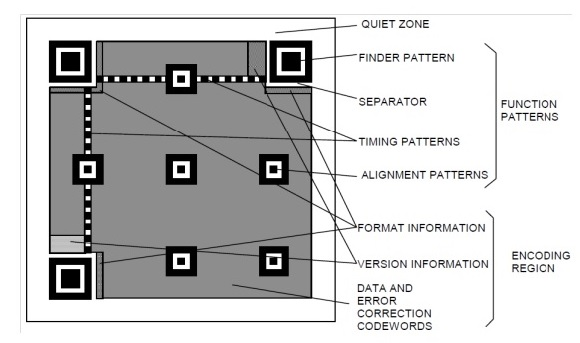
\includegraphics[width=1\textwidth]{figures/Figure21Version7QR.jpg}
    \label{fig:21}
\end{figure}

It is worth mentioning that the Figure \ref{fig:21} is a general format and is not necessary belongs to version 7. It can be present some other versions but it definitely demonstrates the general format of version 7 QR symbol. 

\section{Function Patterns}
"Encoding Regions" are related to the generation and decoding or QR symbol while "Function Patterns" are related to pattern recognition and scene understanding parts.\\
Function patterns are used for the Pattern Recognition and finding the location of the QR symbol and determining its
characteristics, in order to reconstruct the QR-Matrix for decoding process. Function patterns are not related to decoding message. QR-Matrix is simply consider a black module as 0 and a white module as 1. so the QR matrix of the version 1 is $21 \times 21$. More discussion about QR-Matrix would be provided in the subsequent sections Module positions form the QR-Matrix and defined by their row and column coordinates in the symbol, in the form (i, j) where i represents the row (top-down order) and j the column (left-right order) in which the module is located, with counting beginning at 1. Module (1, 1) is therefore located at the upper left corner of the symbol\cite{Thonky}.

\subsection{Finder Patterns}

There is only three \textbf{finder patterns} and are located at exactly three position of the symbol. The upper left, upper right and lower left corners of the symbol. Each finder pattern can be viewed as three concentric squares and is constructed of a black(dark) $7 \times 7$ modules, white(light) $5 \times 5$ modules and finally a dark $3 \times 3$ modules. The wideness ratio of alternative black and white module widths in each finder pattern is approximately 1:1:3:1:1 from any direction (the ratio might be exactly 1:1:3:1:1 depends on the view angle or direction.
This important characteristic help us two find the locations(locations of the centers) of the finder patterns. \textbf{The separator pattern} is a function pattern of all white(light) modules(It is a one module wide) that play the role of a border between the finder patterns and the data region of
the symbol.

\subsection{Alignment Patterns}

The alignment patterns are placed at some specific positions for each particular version, and allow the QR decoder to tolerate distortions when the code is distorted. Except for version 1, other versions have alignment patterns and the number of alignment pattern differ from version to version. Alignment patterns are similar to finder patterns Except for the ratio which is 1:1:1:1:1. The alignment patterns are placed in fixed positions that are defined in the standard \cite{1iso}.

\subsection{Timing Patterns}

The timing patterns are two alternating sequences of black and white modules determining module coordinates in the symbol. Their place is specific in the symbol; the horizontal timing pattern is along with the sixth row of the symbol
between the separators for the two upper finder patterns and the vertical timing pattern is along with the sixth column of the symbol between the separators of the top-left and bottom-left finder patterns. For better understanding, let's scan the sixth row(left to right) in the symbol which contains finder patters, separators and timing patterns. The first 7 modules are belong to top-left finder pattern. The 8th module is white which belongs to separator. Now let's scan this row from right to left. Again the first 7 modules are belong to right-left finder pattern. The 8th module is white which belongs to the other separator. Now the other modules in this row belongs to horizontal timing pattern which its length is:
$$Version*4+17-16=Version*4+1$$
Same procedure applied for vertical timing pattern and the lengths are the same.

\section{Encoding Region and Generating QR Symbol}\label{Encod}

If a region is not related to function patterns is related to data and is available for encoding and error correction, format and version information. The following subsections will explain the QR code encoding process in detail. Here is a general overview of the process which is necessary to understand before going through the encoding process\cite{Thonky}:

\textbf{Step 1: Data and Information Analysis}
The QR-Code generating process, encodes a message or in other word a sequence. There is four available modes for encoding text is QR standard: numeric, alphanumeric, byte, and Kanji. Each mode encodes the text as a sequence of bits (1s and 0s) which different method, and the goal is to produce the shortest possible sequence of bits. Consequently, the first step is to perform data analysis to determine which one of the four modes is optimal for your text.\\

\textbf{Step 2: Data Encoding}
After selecting the encoding mode, the next step is simply Encoding!! In the data encoding subsection this process is described is detail for each encoding mode. The result of this step is a sequence of bits that is split up into data codewords that are each 8 bits long.\\

\textbf{Step 3: Error Correction Coding}
QR codes use error correction in order to tolerate likely damages of image i.e. losing information. This means that after crating the sequence of data bits, error correction codewords should be generated using Reed-Solomon error correction. QR reading both the data codewords and the error correction codewords and comparing them, we're able to determine/correct errors.

\textbf{Step 4: Structure Final Message}
The generated data and error correction codewords, must be arranged in the appropriate order. For large QR codes, the data and error correction codewords are generated in blocks, and these blocks must be interleaved according to the QR code specification.\\

\textbf{Step 5: Module Placement in Matrix}
After generating the data codewords and error correction codewords and arranging them in the correct order, you must place the bits in the QR code matrix. The codewords are arranged in the matrix in a specific way. During this step, you will also place the patterns that are common to all QR codes, such as the boxes on the three corners.\\

\textbf{Step 6: Data Masking}
Certain patterns in the QR code matrix can make it difficult for QR code scanners to correctly read the code. To prevent this, the QR code specification defines eight mask patterns, each of which changes the QR code according to a particular pattern. You must determine which of these mask patterns results in the QR code with the fewest undesirable traits. This is done by evaluating each masked matrix based on four penalty rules. Your final QR code must use the mask pattern that resulted in the lowest penalty score.\\

\textbf{Step 7: Format and Version Information}
The final step is to add format and (if necessary) version information to the QR code by adding pixels in particular areas of the code that were left blank in previous steps. The format pixels identify the error correction level and mask pattern being used in this QR code. The version pixels encode the size of the QR matrix and are only used in larger QR codes.\\

\subsection{Data and Information Analysis}
The four encoding modes include the following characters:

\textbf{Numeric mode} is for decimal digits 0 through 9.

\textbf{Alphanumeric mode} is for the decimal digits 0 through 9, as well as uppercase letters (not lowercase!), and the symbols $\$, \%, *, +, -, ., /,$ and : as well as a space.

\textbf{Byte mode}, by default, is for characters from the ISO-8859-1 character set.

\textbf{Kanji mode} is for double-byte characters from the Shift JIS character set. While UTF-8 can encode Kanji characters, it must use three or four bytes to do so. Shift JIS, on the other hand, uses just two bytes to encode each Kanji character, so Kanji mode compresses Kanji characters more efficiently. If the entire input string consists of characters in the double-byte range of Shift JIS, use Kanji mode. It is also possible to use multiple modes within the same QR code.

\subsubsection{How to Choose the Most Efficient Mode}

To select the most efficient mode for the QR code, The characters in the input string and the following conditions should be checked:

If the input string only consists of decimal digits (0 through 9), use numeric mode.\\

If numeric mode is not applicable, and if all of the characters in the input string can be found in the alphanumeric table, use alphanumeric mode. \emph{letters CANNOT be encoded in alphanumeric mode; only uppercase.}\\

If there is a character that is not in the alphanumeric table but can be encoded in ISO 8859-1, use byte mode. As mentioned above, QR code readers may be able to recognize UTF-8 in byte mode.\\


\subsection{Data Encoding}
Each encoding mode is aimed to create the string of bits for the characters that are used in the specific mode. Each mode uses a different method for encoding data into bits.

\subsubsection*{Step 1: Choose the Error Correction Level} 

Before encoding the data, an error correction level should be chosen. QR codes use Reed-Solomon error correction. This process creates error correction codewords based on the encoded data. Error correction is determined for first detecting the error and second correcting it. Since Reed-Solomon coding is a symmetric coding, the error correction codewords simply will be followed by the data codewords. There are four levels of error correction: L, M, Q, H. Table \ref{table2.1} demonstrates the levels and their corresponding error correction capabilities:

\begin{table}[h!]
  \centering
          \caption{Error Correction Table}
         \label{table2.1}
    \begin{tabular}{| l | l |}
    \hline
    Error Correction Level & Error Correction Capability \\ \hline
    L & 7\% data recovery  \\ \hline
    M & 15\% data recovery  \\ \hline
    Q & 25\% data recovery \\ \hline
    H & 30\% data recovery \\ \hline
    \end{tabular}

\end{table}

Error correction penalize the system design and rate which means that it increase the complexity and the number of required bits.

\subsubsection*{Step 2: Determine the Smallest Version for the Data}

As we described before, the different sizes of QR codes are called versions. Each version is 4 pixels larger than the previous version. Each version has a maximum capacity, depending on the mode in use. In addition, the error correction level further restricts the capacity . The character capacities table lists \cite{1iso} the capacities of all QR versions for a given encoding mode and error correction level.

\textbf{How to Determine the Smallest Version}\\
At this point, count the number of characters to be encoded, and determine which is the smallest version that can contain that number of characters for the encoding mode and desired error correction level.

For example, the phrase "HELLO WORLD" has 11 characters. If encoding it with level Q error correction, since a version 1 code using level Q error correction can only contain 10 characters in alphanumeric mode\footnote{According to the character capacities table}, Therefore, the smallest version that can be used in this case is version 2.

\subsubsection*{Step 3: Add the Mode Indicator}


The encoded data must start with the corresponding mode indicator that specifies the mode being used for the subsequent bits that come after it. Table \ref{table2.2} lists the mode indicators for each mode. For example, Since encoding "HELLO WORLD" in alphanumeric mode, the encoded data must start with 0010.

\begin{table}[h!]
  \centering
          \caption{Mode Indicator Table}
         \label{table2.2}
    \begin{tabular}{| l | l |}
    \hline
    Mode name & Mode indicator \\ \hline
    Numeric Mode & 0001  \\ \hline
    Alphanumeric Mode & 0010  \\ \hline
    Byte Mode & 0100  \\ \hline
    Kanji Mode & 1000  \\ \hline
    \end{tabular}

\end{table}

\subsubsection*{Step 4: Add the Character Count Indicator}

\emph{The character count indicator is a sequence of bits that shows the number of characters that are being encoded}. The character count indicator must be placed after the mode indicator. Furthermore, the character count indicator must be a certain number of bits long, depending on the QR version.

Count the number of characters in the original input text, then convert that number into binary. The length of the character count indicator depends on the encoding mode and the QR code version that will be in use. To make the binary string the appropriate length, we need to zero-padding at the left.

The following lists contain the sizes of the character count indicators for each mode and version. For example, if encoding "HELLO WORLD" in a version 1 QR code in alphanumeric mode, the character count indicator must be 9 bits long. The character count of HELLO WORLD is 11. In binary, 11 is 1011. Pad it on the left to make it 9 bits long: 000001011. Put this after the mode indicator from step 3 to get the following bit string: 0010 000001011

\textbf{Versions 1 through 9}\\
Numeric mode: 10 bits\\
Alphanumeric mode: 9 bits\\
Byte mode: 8 bits\\
Japanese mode: 8 bits\\
\textbf{Versions 10 through 26}\\
Numeric mode: 12 bits\\
Alphanumeric mode: 11 bits\\
Byte mode: 16\\
Japanese mode: 10 bits\\
\textbf{Versions 27 through 40}\\
Numeric mode: 14 bits\\
Alphanumeric mode: 13 bits\\
Byte mode: 16 bits\\
Japanese mode: 12 bits\\

Since we only consider version 1 through 6 in this project, the numbers for version 1 through 9 would applied.

\subsubsection*{Step 5: Encode Using the Selected Mode}

The previous section, data analysis, explains how to select the appropriate encoding mode for a given string. The process for each encoding mode is explained in\cite{Thonky}.

\subsubsection*{Step 6: Break Up into 8-bit Codewords and Add Pad Bytes if Necessary}


After obtaining a string of bits that consists of the mode indicator, the character count indicator, and the data bits as described in steps 1 through 3, it may be necessary to add 0s and pad bytes, because the QR code standard specification requires that the bit string must completely fill the total capacity of the QR code.

\textbf{Determine the Required Number of Bits for this QR Code}\\
To determine how many data bits are required for a particular QR code, refer to the \cite{1iso}. Find the version and error correction level that is in use for the QR code being encoded, and find the number in the column that is labeled "Total Number of Data Codewords for this Version and EC Level". Multiply this number by 8 to obtain the total number of data bits required for this version and error correction level.

For example, according to the table, a version 1-Q code has 13 total data codewords. Therefore, the total number of bits required for this QR code is 13 * 8, or 104 bits.

\textbf{Add a Terminator of 0s if Necessary}\\
If the bit string is shorter than the total number of required bits, a terminator of up to four 0s must be added to the right side of the string. If the bit string is more than four bits shorter than the required number of bits, add four 0s to the end. If the bit string is fewer than four bits shorter, add only the number of 0s that are needed to reach the required number of bits.

For example, if encoding HELLO WORLD in a version 1-Q QR code, the total number of required bits is 104 bits. The data bit string is 74 bits long. The terminator must only be at most 4 bits long, so add four 0s to the right of the string. The resulting string is still too short to fill the 104 bit capacity, but the QR code specification requires that the terminator be at most four 0s in length. If the string had been 102 bits instead, the terminator would only be 2 bits in length.

\textbf{Add More 0s to Make the Length a Multiple of 8}\\
After adding the terminator, if the number of bits in the string is not a multiple of 8, first pad the string on the right with 0s to make the string's length a multiple of 8.

For example, after adding the terminator to the HELLO WORLD string, the length became 78 bits long. This is not a multiple of 8. The bit string is shown here broken up into 8-bit binary bytes:
00100000 01011011 00001011 01111000 11010001 01110010 11011100 01001101 01000011 010000

There are six bits at the end. Add two 0s to make it an 8-bit binary byte:

00100000 01011011 00001011 01111000 11010001 01110010 11011100\\ 01001101 01000011 010000\textbf{00}

\textbf{Add Pad Bytes if the String is Still too Short}\\
If the string is still not long enough to fill the maximum capacity, add the following bytes to the end of the string, repeating until the string has reached the maximum length:
11101100 00010001

These bytes are equivalent to 236 and 17, respectively. They are specifically required by the QR code specification to be added if the bit string is too short at this stage.

For example, the HELLO WORLD string above is 80 bits long. The required capacity for a 1-Q code, as stated earlier on the page, is 104 bits. The number of bits that must be added to fill the remaining capacity is 104 - 80, or 24. Divide this by 8: 24 /8 = 3. Therefore, three pad bytes must be added to the end of the data string. This is shown below:
00100000 01011011 00001011 01111000 11010001 01110010 11011100\\ 01001101 01000011 01000000 \textbf{11101100 00010001 11101100}

\subsection{Error Correction Coding}

Error correction coding provides appropriate conditions to extract the correct bit stream and decode the QR-code message in noisy scenarios. In other words if the image is corrupted or blur we may loss information by not correctly detecting the bits. In other scenario some parts of the QR pattern might be unavailable by any reason. The task of error correction decoding is to detect and correct the errors. Reed-Solomon coding is used for QR-code generation. After performing the previous part and transforming each 8-bits to a decimal number, we have decimal sequence. In this part according to this decimal sequence an error correction sequence has to be generated. This error correction sequence is added to the data codewords and they both form another longer decimal sequence. The length of error correction codewords depends on three factors:
\begin{itemize}
\item Length of data sequence
\item Version of QR code
\item Error correction level
\end{itemize}

Remember that in some cases( Different versions and error correction levels) the data would be broken to different sub-blocks and for each of sub-block a unique error correction sequence would be generated. Finally the data and error correction sequences will be interleaved in some specific order\cite{1iso}.

\subsection{Structure Final message}

In this part the interleaved data and error correction level is ready to form the final message. The decimal sequence now should be transformed to a binary sequence which obviously its length is a multiple of 8. The problem is the QR-Matrix should be fulled. Lots of QR matrices in different version doesn't have 8-divisible module numbers. \emph{So in version 2 through 7 the standard required that 7 reminder bits be added to the end of the generated bit stream}. For version 1 there is no need for any reminder bits.

\subsection{Module Placement in Matrix}

Suppose that after previous steps, Now we have the binary message which we need to put in the QR format. Some consideration are worth to consider. This part dedicated to the method and procedure for placing bit stream into the QR code\cite{Thonky}.

\subsubsection{Review of Function Patterns}

QR codes must include function patterns. These are shapes that must be placed in specific areas of the QR code to ensure that QR code scanners can correctly identify and orient the code for decoding. Figure \ref{fig:22} gives an example of what the function patterns are and where they are positioned. The finder patterns are the three blocks in the corners of the QR code at the top left, top right, and bottom left.

\textbf{The separators} are areas of white-space beside the finder patterns.

\textbf{The alignment patterns} are similar to finder patterns, but smaller, and are placed throughout the code. They are used in versions 2 and larger, and their positions depend on the QR code version.

\textbf{The timing patterns} are dotted lines that connect the finder patterns.

\textbf{The dark module} is a single black module that is always placed beside the bottom left finder pattern.

The sections below explain in greater detail how to position the function patterns. 
\begin{figure}[H]
  \caption{QR symbol\cite{Thonky}}
  \centering
    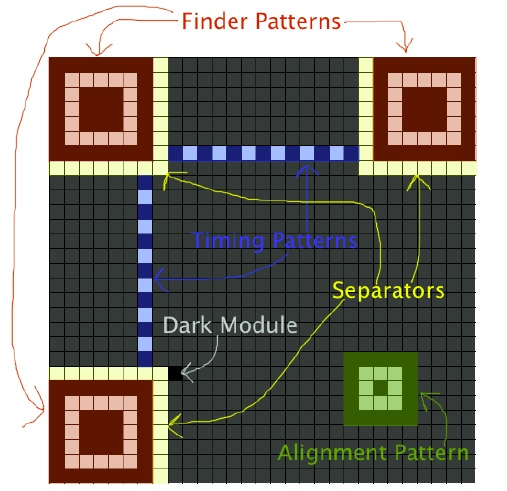
\includegraphics[width=0.4\textwidth]{figures/QR.jpg}
    \label{fig:22}
\end{figure}

Remember that we only consider version 1 through 6 for explaining these parts but also remember that the majority of explanations are the same for higher versions.\\
\\
\subsubsection{Finder Patterns}

 Any finder pattern consists of a square that is 7 modules by 7 modules, an inner white square that is 5 modules by 5 modules, and a full black square in the center that is 3 modules by 3 modules. The finder pattern is a special pattern which is almost impossible to be find in the other parts of the QR-code which is shown is Figure \ref{fig:23}. The module of the finder pattern have a ratio of 1:1:3:1:1. This ration is for alternative black and white modules which stats with black and obviously end by black again.
 
 \begin{figure}[H]
  \caption{Finder Pattern}
  \centering
    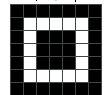
\includegraphics[width=0.3\textwidth]{figures/Finderpattern.jpg}
    \label{fig:23}
\end{figure}

In all versions the finder patterns are placed in the top left, top right, and bottom left corners of the QR code. The finder pattern can be find by the center of its inner solid black square. here are the centers for different finder patterns(first number in the bracket is row and second one is column):

\begin{itemize}
\item \textbf{top-left:} $[4,4]$
\item \textbf{top-right:} $[4,(4*version+17)-3]$
\item \textbf{down-left:} $[(4*version+17)-3,4]$
\end{itemize}

\subsubsection{Separators}

The separators are exactly separator lines of white modules(One module wide) that are placed beside the finder patterns to isolate them from the other of the QR code. The separators are only placed beside the edges of the finder patterns that touch the inside of the QR code. Consider the rounding area of the top-left finder pattern: 
\begin{figure}[H]
  \caption{Separator}
  \centering
    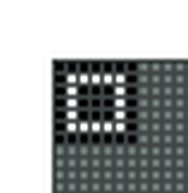
\includegraphics[width=0.3\textwidth]{figures/Separator.jpg}
    \label{fig:24}
\end{figure}


\subsubsection{Alignment Pattern}

QR codes that are version 2 and larger are required to have alignment patterns. An alignment pattern is similar to the finder pattern by the difference in the center square which is only a $1\times1$ black module rather then and $3\times3$ black square.

In version 1 through 6 the alignment patter(its center which is the dark black module) is placed at the $[(4*version+17)-6,(4*version+17)-6]$. As it is obvious from Figure \ref{fig:25} the center of Alignment Pattern is exactly in the column which the left-most black modules of the top-right finder patter exists and also in the row of which the most top black modules of the down-left finder patter exists.
\begin{figure}[H]
  \caption{Alignment Pattern}
  \centering
    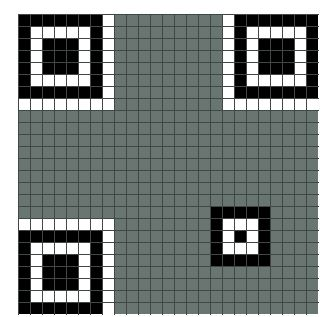
\includegraphics[width=0.3\textwidth]{figures/Alignmentpattern.jpg}
    \label{fig:25}
\end{figure}

\subsubsection{Timing Patterns}

The timing patterns are two horizontal and vertical lines of alternating dark and light modules. The horizontal and vertical timing patterns are placed on the 6th row and 6th column of the QR code respectively between the separators. The timing patterns always start and end with a dark module otherwise it's hard to
realize the starting point of the timing pattern because the separator is white. Figure \ref{fig:26} images show timing patterns on versions 2 through 6.

\begin{figure}[H]
  \caption{Timing Patterns}
  \centering
    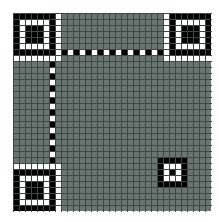
\includegraphics[width=0.5\textwidth]{figures/Timingpattern.jpg}
    \label{fig:26}
\end{figure}

\subsubsection{Dark Module and Reserved Areas}

Before adding the data bits to the QR code matrix, the dark module must be added, and there are areas of the matrix that must be reserved for the format and version bits, which will be added later. All QR codes have a dark module located at the coordinate $([(4 * Version) + 9], 8)$ where V is the version of the QR code. A strip of modules in neighborhoods of the separators must be reserved for the format information area as follows:
\begin{itemize}
\item Near the top-left finder pattern, a one-module strip must be reserved below and to the right of the separator.
\item Near the top-right finder pattern, a one-module strip must be reserved below the separator.
\item Near the bottom-left finder pattern, a one-module strip must be reserved to the right of the separator.
\end{itemize}


Figure \ref{fig:27} demonstrates the framework.
\begin{figure}[H]
  \caption{Reserved Area\cite{Thonky}}
  \centering
    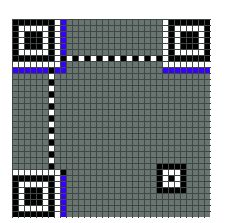
\includegraphics[width=0.5\textwidth]{figures/ReservedArea.jpg}
    \label{fig:27}
\end{figure}

\subsubsection{Placing the Data Bits}

Now we have the data bits and we want to place it in the matrix. Except for the aforementioned function patterns, dark module and reserved area other QR-Matrix entries should be filled with the bit stream which was produced by the data encoding part.
For filling the matrix there is a pattern. 

The data bits are placed beginning at the bottom-right of the matrix and continuing upward in a column that is 2-modules wide. When the column reaches the top, the next 2-module column starts to the left of the previous column and continues downward. Whenever the current column reaches the edge of the matrix, move on to the next 2-module column and reverse direction. If a function pattern or reserved area is reached, the data bit is placed in the next unused module.

The following figure demonstrates this pattern:
Figure \ref{fig:27} demonstrates the framework.
\begin{figure}[H]
  \caption{QR-Matrix Bit Allocating Pattern\cite{Thonky}}
  \centering
    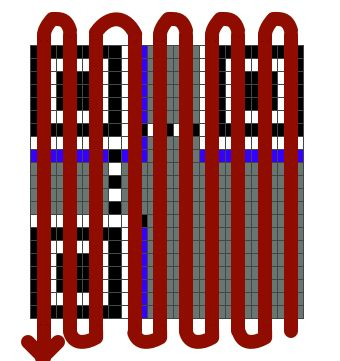
\includegraphics[width=0.5\textwidth]{figures/Feeding.jpg}
    \label{fig:28}
\end{figure}

In the Figure \ref{fig:28} in any 2-module length column there is a pattern for fulfilling the matrix places which is demonstrated in Figure \ref{fig29}.
%%%%%%%%%%%%%%%%
%%%%%%%%%%%%%%%%%%%%%%%%%%%%%%%%%%%%%%%%%
\begin{figure}[ht!]
     \begin{center}
%
        \subfigure[Upward bit allocating]{%
            \label{fig:first}
            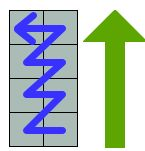
\includegraphics[width=0.4\textwidth]{figures/upwardfeed.jpg}
        }%
        \subfigure[Downward bit allocating]{%
           \label{fig:second}
           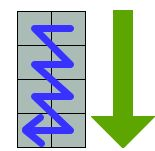
\includegraphics[width=0.4\textwidth]{figures/downwardfeed.jpg}
        }%  ------- End of the first row 
    \end{center}
    \caption{%
The inner pattern for upward and downward bit allocation\cite{Thonky}
     }%
   \label{fig29}
\end{figure}
%%%%%%%%%%%%%%%%%%%%%%%%%%%%%%%%%%%%%%%%%%%%%%%%
%%%%%%%%%%%%%%%%%%%%%%%%%%%%%%%%%%%%%%%%%%%

\subsection{Data Masking}

After placing the bit stream in the QR-Matrix, Now a mask pattern must be applied to the data part in the matrix. Remember that function patterns and other reserved area are not included in the masking procedure. The process of data masking change dark modules to bright and reverse in some specific way. 

There is 8 different mask patterns. Each of them should be applied to the matrix and for any of them a penalty score should be calculated\cite{1iso}. Any of the mask patterns which provides less penalty score is the most appropriate one and it is gonna be chosen. \textbf{Basically mask patterns only applied to data modules and error correction modules}.

\subsection{Format and Version Information}

The final part to generating a quick response code is to create the format and version string and put them in appropriate place in the matrix. There is no version information string in the version 1 through 6 and since we only need to them so we ignore investigating version information allocation.

\subsubsection{Generate the Format String}\label{Format}

The format information string determine which error correction level and which mask pattern have been used in the QR code generation. Since there are four possible error correction levels (L, M, Q, and H) and eight possible mask patterns, there are total of 32 possible format information strings.

The format string is 15 bits long. To create that, a five bit string that shows the error correction level and the mask pattern in QR code has to be generated. Then by using those five bits to generate ten error correction bits. The resulting fifteen bits are XORed with the bit stream \textbf{101010000010010}. 
Now the next step is to determine how the first five bits is generated. That based on two things: \textbf{the first two bits show error correction level and  subsequent three bits show the number of mask pattern.}

\textbf{Error Correction Bits}\\

The first step is to get the two bits that specify the error correction level. The table \ref{table2.3} contains the bit sequences for each error correction level. 

\begin{table}[h!]
  \centering
          \caption{The Error Correction Bits}
         \label{table2.3}
    \begin{tabular}{| l | l |}
    \hline
    EC Level & bits \\ \hline
    L & 01  \\ \hline
    M & 00  \\ \hline
    Q & 11 \\ \hline
    H & 10 \\ \hline
    \end{tabular}

\end{table}

\textbf{Mask Patterns Bits}\\

For the mask patterns table \ref{table2.4} shows the mask number that goes with each pattern and Converting the number into a three-bit binary is the final result for mask pattern bits.

\begin{table}[h!]
  \centering
          \caption{The Mask Pattern Bits}
         \label{table2.4}
    \begin{tabular}{| l | l |}
    \hline
    Number & If true switch the bit \\ \hline
    0 & (row + column) mod 2 == 0  \\ \hline
    1 & (row) mod 2 == 0  \\ \hline
    2 & (column) mod 3 \\ \hline
    3 & (row + column) mod 3 \\ \hline
    4 & ( floor(row / 2) + floor(column / 3) ) mod 2 \\ \hline
    5 & ((row * column) mod 2) + ((row * column) mod 3) == 0)  \\ \hline
    6 & ( ((row * column) mod 2) + ((row * column) mod 3) ) mod 2 == 0 \\ \hline
    7 & ( ((row + column) mod 2) + ((row * column) mod 3) ) mod 2 == 0 \\ \hline
    \end{tabular}

\end{table}

Now by using five bits for the format string, ten error correction bits should be generated. So finally there is a 15 bits binary sequence. This should be XORed with the bit stream \textbf{101010000010010} and the final 15 bits stream should be placed in the QR matrix as below:


\begin{figure}[H]
  \caption{Format Information Data\cite{Thonky}}
  \centering
    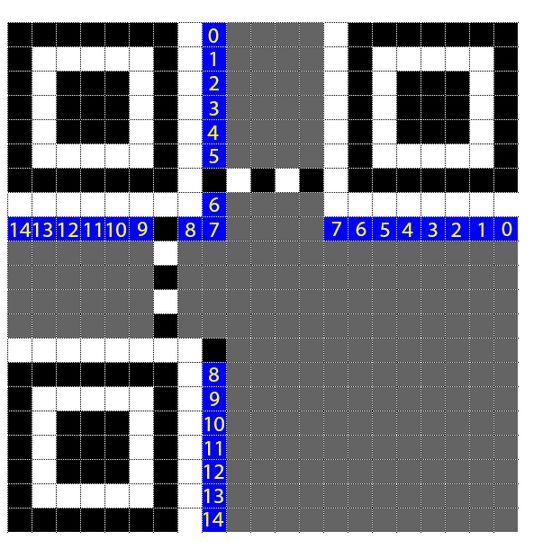
\includegraphics[width=0.5\textwidth]{figures/Formatinformation.jpg}
    \label{fig:2.10}
\end{figure}

The most significant bit of the stream will be placed in place number 14 and as a descending order the least significant bit will be placed in the place number 0.

Now the QR-Matrix is full and in other word the QR-code has been generated.

 % QR Code Structure
\clearpage

\lhead{\emph{Image Processing and Pattern Recognition}}
\chapter{Image Processing and Pattern Recognition}

In this chapter the image processing needed to pattern recognition and extract the exact QR-Code matrix. For this purpose, MATLAB is used, under the license provided by the University of Maryland College Park.


The procedure of detecting the image is explained in detail here and an excerpt of code script provided for better explanation. The overall flowchart for this section is as the image in the next page. The Reed-Solomon Decoder and message extraction box would be explained later. 


\tikzstyle{decision} = [diamond, draw, fill=blue!20, 
    text width=4.5em, text badly centered, node distance=3cm, inner sep=0pt]
\tikzstyle{block} = [rectangle, draw, fill=blue!20, 
    text width=5em, text centered, rounded corners, minimum height=4em]
\tikzstyle{line} = [draw, -latex']
\tikzstyle{cloud} = [draw, ellipse,fill=red!20, node distance=3cm,
    minimum height=2em]
    
\begin{tikzpicture}[node distance = 3cm, auto]
    % Place nodes
    \node [cloud] (expert) {Image};
    \node [block, below of=expert](init) {Image to binary};
    \node [cloud, right of=init, node distance=4cm] (system) {Version Num};
    \node [block, below of=init] (identify) {Median filter};
    \node [block, below of=identify] (evaluate) {Find three finder pattern};
    \node [block, left of=evaluate, node distance=4cm] (update) {Change im2binary threshold/Stop};
    \node [decision, below of=evaluate, node distance=4cm] (decide) {is there three finder pattern?};
    \node [block, below of=decide, node distance=4cm] (AP) {Find alignment pattern};
    \node [decision, right of=AP, node distance=5cm] (FindAP) {is there any alignment pattern?};
    
    \node [block, right of=FindAP, node distance=5cm] (Geo1) {Geo Trans using 3 FP and 1 AP};
    \node [block, below of=FindAP, node distance=5cm] (Geo2) {Geo Trans using 3 FP and the last corner};
    \node [block, above of=Geo1, node distance=3cm,text width=4cm] (Crop) {Extract the QR-Code exact image};
    \node [block, above of=Crop, node distance=4cm,text width=4cm] (FF) {Reed-Solomon Decoder/Message Extraction};
    % Draw edges
    \path [line] (init) -- (identify);
    \path [line] (identify) -- (evaluate);
    \path [line] (evaluate) -- (decide);
    \path [line] (decide) -| node [near start] {No} (update);
    \path [line,dashed] (update) |- (init);
    \path [line] (decide) -- node {Yes}(AP);
    \path [line,dashed] (expert) -- (init);
    \path [line,dashed] (system) -- (init);
    \path [line,dashed] (system) |- (evaluate);
    \path [line] (AP) -- (FindAP);
    \path [line] (FindAP) -- node{Yes}(Geo1);
    \path [line] (FindAP) -- node{No}(Geo2);
    \draw[ultra thick, blue, ->]  
    (Geo1) -- (Crop);
    \draw[ultra thick, blue, ->]  
    (Geo2) -- (Crop);
    \draw[ultra thick, red, ->]  
    (Crop) -- (FF);

   
\end{tikzpicture}


\section{Preprocessing}

\subsection{Image Transformation}

For the thresholding and creating a binary image, a sub-function named \textbf{$"im2binary\_Fn"$} has been design and implemented. This sub function get the image and using some thresholding return the black and white image. This is enough for QR-code because it only contains dark and bright modules which are binary $1$ and $0$ respectively. The script is as below:
\begin{lstlisting}
function Im_binary = im2binary_Fn(img,Thresh)
% Find the gray threshold level
if isempty(Thresh)
    Th = graythresh(img);
else
    Th = graythresh(img)-Thresh;
end
% Make the image binary using the level
Out = im2bw(img,Th);
Im_binary=Out;
\end{lstlisting}

\subsection{Median Filtering}

The reason of median filtering is that sometimes in the process of thresholding and creating a binary data from an image, patterns like salt and pepper noise might be produced. Median filtering is a powerful simple method to avoiding that flaw. The script is as simple as $ medfilt2(img)$. In order to better filtering one can use the different window sizes for the MATLAB function.

\section{Finding and Locating the Finder Patterns}

After thresholding and median filtering, the next task is to detect the QR code pattern from the image. For
this, we need to locate where the QR code is in the image and then reconstruct only the QR code part. The first major step is to finding three FPs\footnote{Finder Patterns}. According to the international
standard of QR code encoding \cite{1iso} and as we mentioned earlier, the ratio between the black and white modules in the
finder patterns is 1:1:3:1:1 which starts and ends with black. For finding finder pattern a horizontal and vertical search will be enough because from any point of view the aforementioned ratio is fixed with some tolerance coefficient. Sub-function $"find\_Probable\_FIPs\_Fn"$ use the following procedure for finding a finder pattern:

\textbf{Step1:}\\ Scan each row of the image and save the length of the black and white modules(How many successive pixels in a row have the same color). Sub-function $"Mod\_Tr\_Fn"$ detect the successive color order in a row matrix.

\begin{lstlisting}
for row = 1 : row_Num
        Tr_Line = img(row,:); % pick out the entire row
        
        % calculate the appearence of the modules in row.
        length_modules = Mod_Tr_Fn(Tr_Line);
end
\end{lstlisting}

Figure \ref{fig:3.1} demonstratess the row and column scanning.

\begin{figure}[H]
  \caption{Row and Column scanning for FPs locating}
  \centering
    
\includegraphics[width=0.5\textwidth]{figures/rowcolumnscan.jpg}
    \label{fig:3.1}
\end{figure}

\textbf{Step2:}\\ Consider every consecutive 5 elements of this length module of the row and calculate and extract the ratio of it.

\begin{lstlisting}
        for i = 1:length(length_modules)-4  
            vectorFIP = length_modules(i:i+4);
        end
\end{lstlisting}

\textbf{Step3:}\\ Check the ratio to see whether it is 1:1:3:1:1 or not. Also check to see that the first module is black or not. The sub-function $"checkRatio\_Fn"$ has been defined for checking the desired ration.

\begin{lstlisting}
[isFIP, ~] = checkRatio_Fn(vectorFIP, [1 1 3 1 1]);
            if(isFIP &&  img(row, pixelPosCol)==0)
\end{lstlisting}

\textbf{Step4:}\\ If the ratio is correct, the center position of the finder pattern which is the middle black block is found and save the length of the successive black and white modules in that column. Repeat step-2 and step-3 for the column.

\begin{lstlisting}
            if(isFIP &&  img(row, pixelPosCol)==0)
                col = pixelPosCol + floor(sum(vectorFIP)/2);
                pixelPosRow=1; %  Initial point
              
                Tr_col = Mod_Tr_Fn(img(:,col));
                 for j = 1:length(Tr_col)-4
                    vector_row_FIP = Tr_col(j:j+4);
                    [rowFIP, ~] =  checkRatio_Fn(vector_row_FIP, [1 1 3 1 1]);
                 end
                    
\end{lstlisting}




\textbf{Step5:}\\ One more time find the center position of the finder pattern in the column and check whether this point is over the previous center point or not. If the answer is yes so the center if found. If no, Ignore this row and check next row. 

\begin{lstlisting}
                    if(rowFIP && img(pixelPosRow,col)==0)
                        rows = pixelPosRow + sum(vector_row_FIP)/2;
                        if (abs(rows-row) <= 8) 
                            numberOfFIPS = numberOfFIPS + 1;
                            locationFIPs = [locationFIPs; [row col]];
                        end
                    end 
                    
\end{lstlisting}

\textbf{Note that the command $"if (abs(rows-row) <= 8)"$ is for a tolerance in coincidence of the row and column for finding the center}. We consider the number of 8. One can consider number of 1 for example. This factor if high let us consider more points as FIP candidates because is harsh situation which the image is very blurred or distorted, if the number of pixels is high even the finding of Finder Patterns would be difficult if the image is not straight because we cannot detect the correct ration.

\textbf{Step6:}\\ In the previous steps some finder patterns has been find as candidates. But we want to choose three of them which correspond to the main three finder patterns. The sub-function $"findFIP\_Order\_Fn"$ has been developed for doing that. The first part of it is to clustering which is an unsupervised learning using a famous pattern recognition MATLAB function which automatically divide the area into three category.

\begin{lstlisting}
    if( length(FIP) > 2 )

        [idx, Points] = kmeans(FIP,3,'Distance','cityblock',...
                           'Replicates',5)  ;    

        for i=1:3       
            Pos = Points(i,:);
            Determnd_Location = FIP(idx==i,:);       
            [~,index] =min( pdist2( Pos, Determnd_Location, 'euclidean') );
            FIPs(i,:)=Determnd_Location(index,:); 
        end
     end
                    
\end{lstlisting}

Then by searching the three cluster using the developed algorithm, three of them will be chosen. These three are the finder patterns.


\textbf{Step7:}\\ The last part is to extract the order of finder patterns because we now have the three finder patterns but we don't know which one is for example the top-left finder pattern or which one is the top-right. The sub-function $"get\_Correct\_Order\_FIPs\_Fn(FIPs)"$ in the last part of The sub-function $"findFIP\_Order\_Fn"$ performs this task. The following semi-pseudo code shows that:

\begin{lstlisting}
switch Max_indx
    Find A(pseudo code)
    AB = B-A;
    AC = C-A;
    %BC = C-B;
    k = AB(1)*AC(2) - AB(2)*AC(1);
    if k > 0
        C_point = C;
        B_point = B;
    else
        B_point = C;
        C_point = B;
    end
                    
\end{lstlisting}

Now lets have examples of finding finder patterns. the following figures show the locating of the finder pattern.
\begin{figure}[H]
  \caption{Finder pattern recognition of a damaged image}
  \centering
    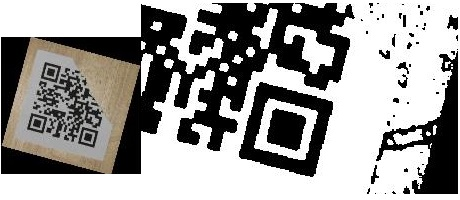
\includegraphics[width=0.9\textwidth]{figures/finderpattern1.jpg}
    \label{fig:3.2}
\end{figure}

\begin{figure}[H]
  \caption{Finder pattern recognition of QR-art}
  \centering
    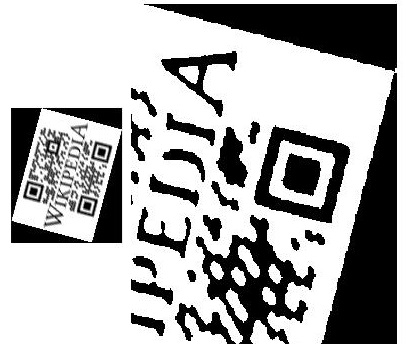
\includegraphics[width=0.9\textwidth]{figures/finderpattern2.jpg}
    \label{fig:3.3}
\end{figure}

\begin{figure}[H]
  \caption{Finder pattern recognition of distorted image}
  \centering
    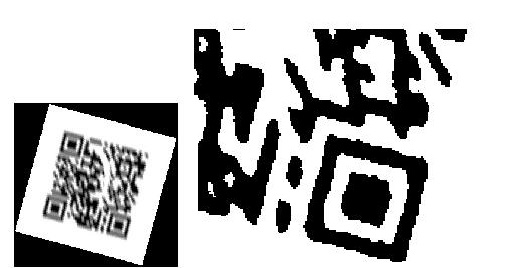
\includegraphics[width=0.9\textwidth]{figures/finderpattern3.jpg}
    \label{fig:3.4}
\end{figure}

\section{Finding the Alignment pattern Patterns}

After locating the finder patterns, the next task is to detect and locate the alignment pattern. For
this, we need to locate where the rounding area of AP\footnote{Alignment Pattern} is in the image and then search for the specific pattern. According to the standard of QR code \cite{1iso} the ratio between the black and white modules in the
AP is 1:1:1:1:1 which starts and ends with black. 

For finding finder pattern, in contrast with the FPs, a horizontal and vertical search will not be necessary enough because the algorithm may find such patterns in the image which are not any alignment patterns. Sub-function $"findAP\_Fn"$ use the following procedure for finding a finder pattern:

\textbf{Step1:}\\ The horizontal and vertical searching are exactly like the ones for locating finder patterns but the difference is that the ratio of 1:1:1 is considered to be searched. \textbf{Note that we do not search for ratio 1:1:1:1:1 because there is no separator for alignment pattern so we use the outer black square of the AP as a separator}.



\textbf{Step2:}\\ The previous step finds some candidates for being AP. This step performs a diagonal search for validating the candidates and ignore any candidate which does not have the ratio 1:1:1 from its diagonal point of view. Figure demonstrates the extra diagonal search. Sub-function $"check_AP_Fn"$ tries to validate different Alignment Patterns by diagonal search

\begin{lstlisting}
for i=1:size(locationAP,1)
    AP=locationAP(i,:);
    [ answer ] = check_AP_Fn( AP,img);
    if ~isempty(answer)
        APnew=[APnew;AP];
    end
end
                   
\end{lstlisting}

Sub-function $"check\_diag\_Fn"$ use the algorithm of diagonal search for checking the diagonal ratio.

\begin{lstlisting}
function answer = check_diag_Fn(AP,range,img)
Vec=[];
for i=-range:1:range
    Vec=[Vec img(AP(1,1)+i,AP(1,2)+i)];
end
length_modules = Mod_Tr_Fn(Vec);
c=1;
pos=[];
for k = 1:length(length_modules)-2
    row=sum(length_modules(1,1:k-1))+1;
    vectorAP = length_modules(k:k+2);
    [isAP, ~] = checkRatio_Fn(vectorAP, [1 1 1]);
    if (isAP && img(AP(1,1)-range+row-1,AP(1,2)-range+row-1)==1)
        pos(c) = sum(length_modules(1,1:k))+(length_modules(1,k+1))/2;
        c=c+1;
    end
end            
\end{lstlisting}

Basically we ignore the position if the radio of 1:1:1 cannot be detected there and/or the first module is not white(Remember that the black rounding square is used as separator).

Now its time to see some results. Recall that if the algorithm can find alignment pattern then it can plot it.

\begin{figure}[H]
  \caption{Finding Alignment pattern}
  \centering
    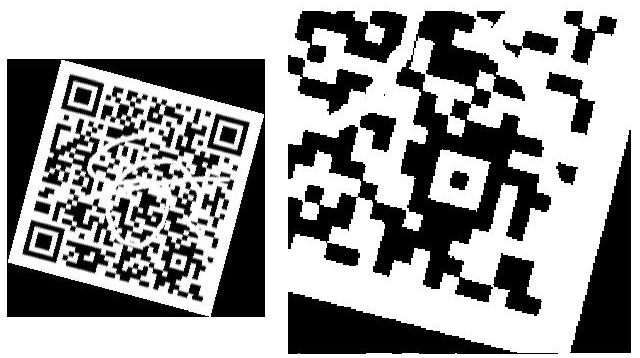
\includegraphics[width=0.9\textwidth]{figures/alignmentpattern1.jpg}
    \label{fig:3.5}
\end{figure}

\section{Geometric Modification}

Geometric Modification is necessary, since the image of the QR code may be distorted, blurred or damaged by any definition. The image must be deblurred and transformed a square pattern. At least 4-points(linearly independent) is needed to successfully perform geometric transformation. Two different approaches have been tried.

In the first approach, three finder pattern and the alignment pattern is used to geometrically transform the image. The approach has been developed for any version. But the necessary input is the version number. Figure \ref{fig:3.6} shows the approach.

\begin{figure}[H]
  \caption{Critical point detection}
  \centering
    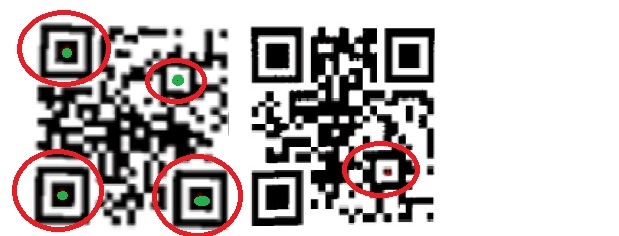
\includegraphics[width=0.9\textwidth]{figures/GeoAP.jpg}
    \label{fig:3.6}
\end{figure}

The next approach which is less precise compared to the previous one, is two find the fourth corner of the QR-code and use that point in staid of Alignment Pattern. This approached is applied when the algorithm cannot detect the center of Alignment Pattern which is possible in very distorted or blurred images.
By using the following code, the other extra points can be calculated and the fourth corner will be extracted to be used for perspective transformation.
\begin{lstlisting}
AC = C-A;
AB = B-A;
P=(B+C)/2;
    
% Find distance between the finder patterns
dist_1 = sqrt(AC(1)^2 + AC(2)^2);
dist_2 = sqrt(AB(1)^2 + AB(2)^2); 
% Difine as the new scale for QR-code reconstruction and is identical in both sides because QR-code pattern is square

cell_width_1=dist_1/(module-7);
cell_width_2=dist_2/(module-7);
normCA=unit_v_Fn(C,A);
normBA=unit_v_Fn(B,A);

%% Extra Points for better reflection
%% Four courners of A
    % A11-------A12
    % |    _/
    % |  _/
    % |_/
    % A21/-------A22

A11 = normCA*((module/2))*cell_width_1 + normBA*((module/2))*cell_width_2 + P;
A22 = normCA*((module/2)-7)*cell_width_1 + normBA*((module/2)-7)*cell_width_2 + P;
A12 = normAC*7*cell_width_1 + A11;
A21 = normAB*7*cell_width_2 + A11;

%% Four courners of B
    % B11-------B12
    % |    _/
    % |  _/
    % |_/
    % B21/-------B22
B11 = normAB*(module-7)*cell_width_2 + A11;
B21 = normAB*(module-7)*cell_width_2 + A21;
B12 = normAB*(module-7)*cell_width_2 + A12;
B22 = normAB*(module-7)*cell_width_2 + A22;

%% Four courners of C
    % C11-------C12
    % |    _/
    % |  _/
    % |_/
    % C21/-------C22

C11 = normAC*(module-7)*cell_width_1 + A11;
C21 = normAC*(module-7)*cell_width_2 + A21;
C12 = normAC*(module-7)*cell_width_2 + A12;
C22 = normAC*(module-7)*cell_width_2 + A22;


MM1= normAB*(module)*cell_width_2 + C12;% The last corener 
MM2= normAC*(module)*cell_width_1 + B21;        
\end{lstlisting}


\subsection{Perspective transformation}

The perspective transformation performs and describes the changes in a perspective projection, when the image is being looked from another point of view\cite{WikiHomo}. Using four point MATLAB can do the task directly. The following image demonstrates an example of perspective transformation.

\begin{figure}[H]
  \caption{Perspective Transformation\cite{StackPers}}
  \centering
    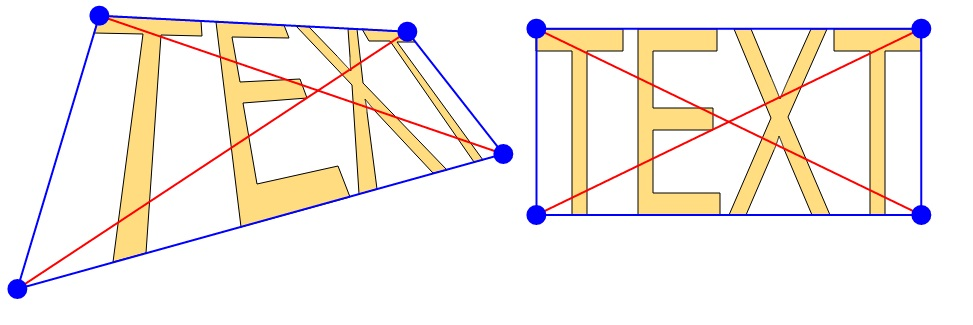
\includegraphics[width=0.9\textwidth]{figures/PersTrans.jpg}
    \label{fig:3.7}
\end{figure}

After finding 4-points which are not linearly dependent, Now we should define the corresponding 4-points to geometrically map the QR-code to a square image. Following code demonstrates the calculation which exactly defines the new corresponding points as "fixed points" and are the Finder patterns and Alignment Pattern places in the standard QR-Matrix which has been defined before.


\begin{lstlisting}

size(ap,2)
if (~isempty(ap) && module>21)      % Versions-1 may not have align pattern
moving_points = [fips(1,2) fips(1,1);            % B position
                    fips(2,2) fips(2,1);            % A position
                        fips(3,2) fips(3,1);        % C position
                            ap(2) ap(1);            % AP 
                            ];

fixed_points = [dist_min dist_fip;
                    dist_min dist_min;
                        dist_fip dist_min;
                              dist_ap dist_ap;
%                              (module)*cell_width (module)*cell_width;
%                              (7)*cell_width (7)*cell_width;
%                              (7)*cell_width (module-7)*cell_width;
%                              (module-7)*cell_width (7)*cell_width;
                            ];

end
       
\end{lstlisting}

Now its the time for MATLAB to transform the perspective by the following prepared function.
\begin{lstlisting}
tform = fitgeotrans(moving_points, fixed_points, 'projective');
newim_S = imwarp(Im, tform, 'linear');
\end{lstlisting}

\subsection{Crop and QR Pattern Demonstration}

After the previous steps, Now we need to crop the QR code pattern from the image and putting it in an exact square form. At first cropping is done by the following part of the program:

\begin{lstlisting}
rect = [FIPLocations(2,2)-(dist_min) FIPLocations(2,1)-(dist_min) side side];
newim = imcrop(newim, rect);
\end{lstlisting}

The using $"imresize"$ function and defining a bigger area(For better demonstration) the QR-code is extracted by the following part of the code:

\begin{lstlisting}
Main_QR_Matrix = imresize(newim, [module module], 'nearest');
Large_QR = imresize(Main_QR_Matrix, [10*module 10*module], 'nearest');
\end{lstlisting}

The following figures show the QR pattern final representation.

\begin{figure}[H]
  \caption{Version-3 QR code recognition}
  \centering
    
\includegraphics[width=0.9\textwidth]{figures/QR1.jpg}
    \label{fig:3.8}
\end{figure}

\begin{figure}[H]
  \caption{Verion-2 QR code}
  \centering
    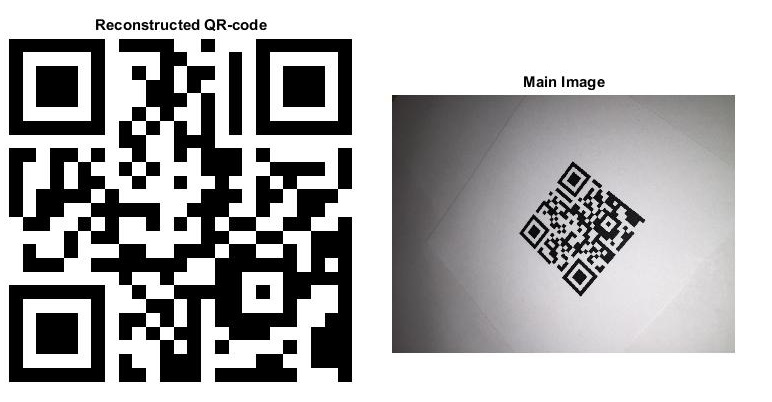
\includegraphics[width=0.9\textwidth]{figures/QR2.jpg}
    \label{fig:3.9}
\end{figure}

\begin{figure}[H]
  \caption{QR code recognition in a high resolution image}
  \centering
    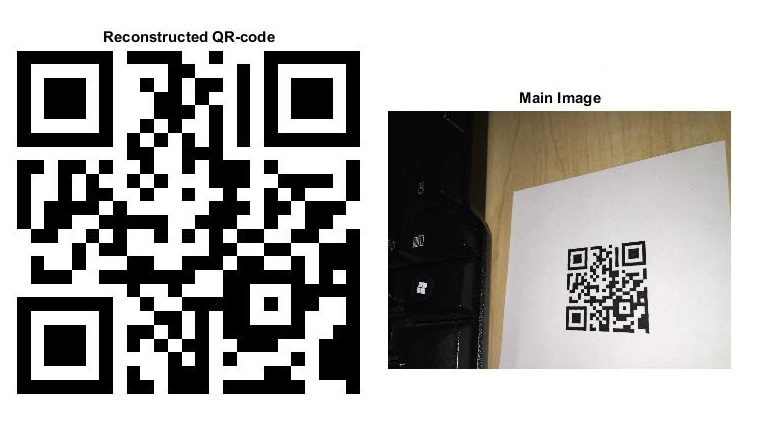
\includegraphics[width=0.9\textwidth]{figures/QR3.jpg}
    \label{fig:3.10}
\end{figure}


This chapter was dedicated to the Image Processing part of the project. In the next chapter decoding of the message will be discussed.







 % QR Code Structure
\clearpage
%\chapter{Image Processing and Pattern Recognition}

In this chapter the image processing needed to pattern recognition and extract the exact QR-Code matrix. For this purpose, MATLAB is used, under the license provided by the University of Maryland College Park.


The procedure of detecting the image is explained in detail here and an excerpt of code script provided for better explanation. The overall flowchart for this section is as the image in the next page. The Reed-Solomon Decoder and message extraction box would be explained later. 


\tikzstyle{decision} = [diamond, draw, fill=blue!20, 
    text width=4.5em, text badly centered, node distance=3cm, inner sep=0pt]
\tikzstyle{block} = [rectangle, draw, fill=blue!20, 
    text width=5em, text centered, rounded corners, minimum height=4em]
\tikzstyle{line} = [draw, -latex']
\tikzstyle{cloud} = [draw, ellipse,fill=red!20, node distance=3cm,
    minimum height=2em]
    
\begin{tikzpicture}[node distance = 3cm, auto]
    % Place nodes
    \node [cloud] (expert) {Image};
    \node [block, below of=expert](init) {Image to binary};
    \node [cloud, right of=init, node distance=4cm] (system) {Version Num};
    \node [block, below of=init] (identify) {Median filter};
    \node [block, below of=identify] (evaluate) {Find three finder pattern};
    \node [block, left of=evaluate, node distance=4cm] (update) {Change im2binary threshold/Stop};
    \node [decision, below of=evaluate, node distance=4cm] (decide) {is there three finder pattern?};
    \node [block, below of=decide, node distance=4cm] (AP) {Find alignment pattern};
    \node [decision, right of=AP, node distance=5cm] (FindAP) {is there any alignment pattern?};
    
    \node [block, right of=FindAP, node distance=5cm] (Geo1) {Geo Trans using 3 FP and 1 AP};
    \node [block, below of=FindAP, node distance=5cm] (Geo2) {Geo Trans using 3 FP and the last corner};
    \node [block, above of=Geo1, node distance=3cm,text width=4cm] (Crop) {Extract the QR-Code exact image};
    \node [block, above of=Crop, node distance=4cm,text width=4cm] (FF) {Reed-Solomon Decoder/Message Extraction};
    % Draw edges
    \path [line] (init) -- (identify);
    \path [line] (identify) -- (evaluate);
    \path [line] (evaluate) -- (decide);
    \path [line] (decide) -| node [near start] {No} (update);
    \path [line,dashed] (update) |- (init);
    \path [line] (decide) -- node {Yes}(AP);
    \path [line,dashed] (expert) -- (init);
    \path [line,dashed] (system) -- (init);
    \path [line,dashed] (system) |- (evaluate);
    \path [line] (AP) -- (FindAP);
    \path [line] (FindAP) -- node{Yes}(Geo1);
    \path [line] (FindAP) -- node{No}(Geo2);
    \draw[ultra thick, blue, ->]  
    (Geo1) -- (Crop);
    \draw[ultra thick, blue, ->]  
    (Geo2) -- (Crop);
    \draw[ultra thick, red, ->]  
    (Crop) -- (FF);

   
\end{tikzpicture}


\section{Preprocessing}

\subsection{Image Transformation}

For the thresholding and creating a binary image, a sub-function named \textbf{$"im2binary\_Fn"$} has been design and implemented. This sub function get the image and using some thresholding return the black and white image. This is enough for QR-code because it only contains dark and bright modules which are binary $1$ and $0$ respectively. The script is as below:
\begin{lstlisting}
function Im_binary = im2binary_Fn(img,Thresh)
% Find the gray threshold level
if isempty(Thresh)
    Th = graythresh(img);
else
    Th = graythresh(img)-Thresh;
end
% Make the image binary using the level
Out = im2bw(img,Th);
Im_binary=Out;
\end{lstlisting}

\subsection{Median Filtering}

The reason of median filtering is that sometimes in the process of thresholding and creating a binary data from an image, patterns like salt and pepper noise might be produced. Median filtering is a powerful simple method to avoiding that flaw. The script is as simple as $ medfilt2(img)$. In order to better filtering one can use the different window sizes for the MATLAB function.

\section{Finding and Locating the Finder Patterns}

After thresholding and median filtering, the next task is to detect the QR code pattern from the image. For
this, we need to locate where the QR code is in the image and then reconstruct only the QR code part. The first major step is to finding three FPs\footnote{Finder Patterns}. According to the international
standard of QR code encoding \cite{1iso} and as we mentioned earlier, the ratio between the black and white modules in the
finder patterns is 1:1:3:1:1 which starts and ends with black. For finding finder pattern a horizontal and vertical search will be enough because from any point of view the aforementioned ratio is fixed with some tolerance coefficient. Sub-function $"find\_Probable\_FIPs\_Fn"$ use the following procedure for finding a finder pattern:

\textbf{Step1:}\\ Scan each row of the image and save the length of the black and white modules(How many successive pixels in a row have the same color). Sub-function $"Mod\_Tr\_Fn"$ detect the successive color order in a row matrix.

\begin{lstlisting}
for row = 1 : row_Num
        Tr_Line = img(row,:); % pick out the entire row
        
        % calculate the appearence of the modules in row.
        length_modules = Mod_Tr_Fn(Tr_Line);
end
\end{lstlisting}

Figure \ref{fig:3.1} demonstratess the row and column scanning.

\begin{figure}[H]
  \caption{Row and Column scanning for FPs locating}
  \centering
    
\includegraphics[width=0.5\textwidth]{figures/rowcolumnscan.jpg}
    \label{fig:3.1}
\end{figure}

\textbf{Step2:}\\ Consider every consecutive 5 elements of this length module of the row and calculate and extract the ratio of it.

\begin{lstlisting}
        for i = 1:length(length_modules)-4  
            vectorFIP = length_modules(i:i+4);
        end
\end{lstlisting}

\textbf{Step3:}\\ Check the ratio to see whether it is 1:1:3:1:1 or not. Also check to see that the first module is black or not. The sub-function $"checkRatio\_Fn"$ has been defined for checking the desired ration.

\begin{lstlisting}
[isFIP, ~] = checkRatio_Fn(vectorFIP, [1 1 3 1 1]);
            if(isFIP &&  img(row, pixelPosCol)==0)
\end{lstlisting}

\textbf{Step4:}\\ If the ratio is correct, the center position of the finder pattern which is the middle black block is found and save the length of the successive black and white modules in that column. Repeat step-2 and step-3 for the column.

\begin{lstlisting}
            if(isFIP &&  img(row, pixelPosCol)==0)
                col = pixelPosCol + floor(sum(vectorFIP)/2);
                pixelPosRow=1; %  Initial point
              
                Tr_col = Mod_Tr_Fn(img(:,col));
                 for j = 1:length(Tr_col)-4
                    vector_row_FIP = Tr_col(j:j+4);
                    [rowFIP, ~] =  checkRatio_Fn(vector_row_FIP, [1 1 3 1 1]);
                 end
                    
\end{lstlisting}




\textbf{Step5:}\\ One more time find the center position of the finder pattern in the column and check whether this point is over the previous center point or not. If the answer is yes so the center if found. If no, Ignore this row and check next row. 

\begin{lstlisting}
                    if(rowFIP && img(pixelPosRow,col)==0)
                        rows = pixelPosRow + sum(vector_row_FIP)/2;
                        if (abs(rows-row) <= 8) 
                            numberOfFIPS = numberOfFIPS + 1;
                            locationFIPs = [locationFIPs; [row col]];
                        end
                    end 
                    
\end{lstlisting}

\textbf{Note that the command $"if (abs(rows-row) <= 8)"$ is for a tolerance in coincidence of the row and column for finding the center}. We consider the number of 8. One can consider number of 1 for example. This factor if high let us consider more points as FIP candidates because is harsh situation which the image is very blurred or distorted, if the number of pixels is high even the finding of Finder Patterns would be difficult if the image is not straight because we cannot detect the correct ration.

\textbf{Step6:}\\ In the previous steps some finder patterns has been find as candidates. But we want to choose three of them which correspond to the main three finder patterns. The sub-function $"findFIP\_Order\_Fn"$ has been developed for doing that. The first part of it is to clustering which is an unsupervised learning using a famous pattern recognition MATLAB function which automatically divide the area into three category.

\begin{lstlisting}
    if( length(FIP) > 2 )

        [idx, Points] = kmeans(FIP,3,'Distance','cityblock',...
                           'Replicates',5)  ;    

        for i=1:3       
            Pos = Points(i,:);
            Determnd_Location = FIP(idx==i,:);       
            [~,index] =min( pdist2( Pos, Determnd_Location, 'euclidean') );
            FIPs(i,:)=Determnd_Location(index,:); 
        end
     end
                    
\end{lstlisting}

Then by searching the three cluster using the developed algorithm, three of them will be chosen. These three are the finder patterns.


\textbf{Step7:}\\ The last part is to extract the order of finder patterns because we now have the three finder patterns but we don't know which one is for example the top-left finder pattern or which one is the top-right. The sub-function $"get\_Correct\_Order\_FIPs\_Fn(FIPs)"$ in the last part of The sub-function $"findFIP\_Order\_Fn"$ performs this task. The following semi-pseudo code shows that:

\begin{lstlisting}
switch Max_indx
    Find A(pseudo code)
    AB = B-A;
    AC = C-A;
    %BC = C-B;
    k = AB(1)*AC(2) - AB(2)*AC(1);
    if k > 0
        C_point = C;
        B_point = B;
    else
        B_point = C;
        C_point = B;
    end
                    
\end{lstlisting}

Now lets have examples of finding finder patterns. the following figures show the locating of the finder pattern.
\begin{figure}[H]
  \caption{Finder pattern recognition of a damaged image}
  \centering
    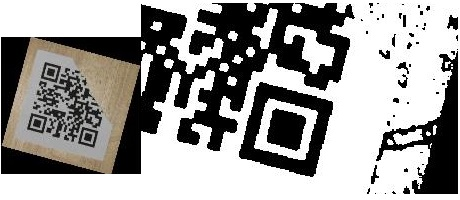
\includegraphics[width=0.9\textwidth]{figures/finderpattern1.jpg}
    \label{fig:3.2}
\end{figure}

\begin{figure}[H]
  \caption{Finder pattern recognition of QR-art}
  \centering
    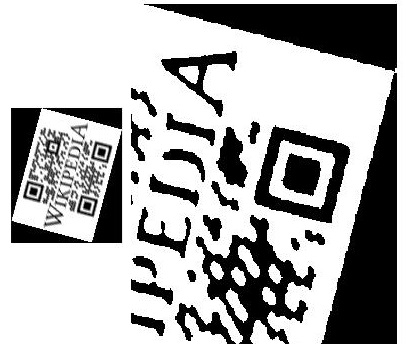
\includegraphics[width=0.9\textwidth]{figures/finderpattern2.jpg}
    \label{fig:3.3}
\end{figure}

\begin{figure}[H]
  \caption{Finder pattern recognition of distorted image}
  \centering
    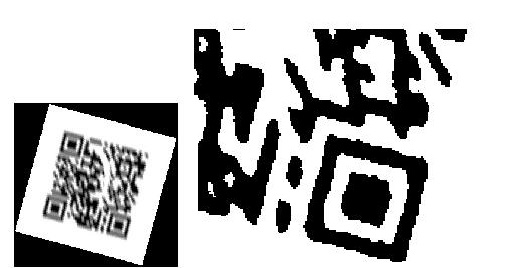
\includegraphics[width=0.9\textwidth]{figures/finderpattern3.jpg}
    \label{fig:3.4}
\end{figure}

\section{Finding the Alignment pattern Patterns}

After locating the finder patterns, the next task is to detect and locate the alignment pattern. For
this, we need to locate where the rounding area of AP\footnote{Alignment Pattern} is in the image and then search for the specific pattern. According to the standard of QR code \cite{1iso} the ratio between the black and white modules in the
AP is 1:1:1:1:1 which starts and ends with black. 

For finding finder pattern, in contrast with the FPs, a horizontal and vertical search will not be necessary enough because the algorithm may find such patterns in the image which are not any alignment patterns. Sub-function $"findAP\_Fn"$ use the following procedure for finding a finder pattern:

\textbf{Step1:}\\ The horizontal and vertical searching are exactly like the ones for locating finder patterns but the difference is that the ratio of 1:1:1 is considered to be searched. \textbf{Note that we do not search for ratio 1:1:1:1:1 because there is no separator for alignment pattern so we use the outer black square of the AP as a separator}.



\textbf{Step2:}\\ The previous step finds some candidates for being AP. This step performs a diagonal search for validating the candidates and ignore any candidate which does not have the ratio 1:1:1 from its diagonal point of view. Figure demonstrates the extra diagonal search. Sub-function $"check_AP_Fn"$ tries to validate different Alignment Patterns by diagonal search

\begin{lstlisting}
for i=1:size(locationAP,1)
    AP=locationAP(i,:);
    [ answer ] = check_AP_Fn( AP,img);
    if ~isempty(answer)
        APnew=[APnew;AP];
    end
end
                   
\end{lstlisting}

Sub-function $"check\_diag\_Fn"$ use the algorithm of diagonal search for checking the diagonal ratio.

\begin{lstlisting}
function answer = check_diag_Fn(AP,range,img)
Vec=[];
for i=-range:1:range
    Vec=[Vec img(AP(1,1)+i,AP(1,2)+i)];
end
length_modules = Mod_Tr_Fn(Vec);
c=1;
pos=[];
for k = 1:length(length_modules)-2
    row=sum(length_modules(1,1:k-1))+1;
    vectorAP = length_modules(k:k+2);
    [isAP, ~] = checkRatio_Fn(vectorAP, [1 1 1]);
    if (isAP && img(AP(1,1)-range+row-1,AP(1,2)-range+row-1)==1)
        pos(c) = sum(length_modules(1,1:k))+(length_modules(1,k+1))/2;
        c=c+1;
    end
end            
\end{lstlisting}

Basically we ignore the position if the radio of 1:1:1 cannot be detected there and/or the first module is not white(Remember that the black rounding square is used as separator).

Now its time to see some results. Recall that if the algorithm can find alignment pattern then it can plot it.

\begin{figure}[H]
  \caption{Finding Alignment pattern}
  \centering
    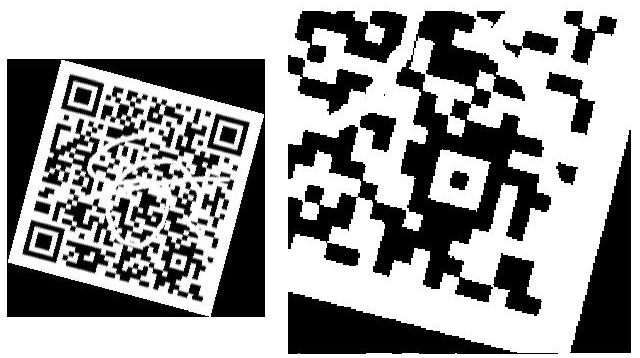
\includegraphics[width=0.9\textwidth]{figures/alignmentpattern1.jpg}
    \label{fig:3.5}
\end{figure}

\section{Geometric Modification}

Geometric Modification is necessary, since the image of the QR code may be distorted, blurred or damaged by any definition. The image must be deblurred and transformed a square pattern. At least 4-points(linearly independent) is needed to successfully perform geometric transformation. Two different approaches have been tried.

In the first approach, three finder pattern and the alignment pattern is used to geometrically transform the image. The approach has been developed for any version. But the necessary input is the version number. Figure \ref{fig:3.6} shows the approach.

\begin{figure}[H]
  \caption{Critical point detection}
  \centering
    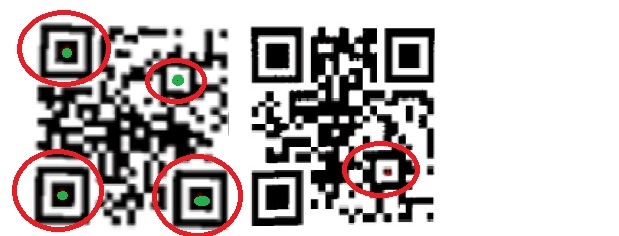
\includegraphics[width=0.9\textwidth]{figures/GeoAP.jpg}
    \label{fig:3.6}
\end{figure}

The next approach which is less precise compared to the previous one, is two find the fourth corner of the QR-code and use that point in staid of Alignment Pattern. This approached is applied when the algorithm cannot detect the center of Alignment Pattern which is possible in very distorted or blurred images.
By using the following code, the other extra points can be calculated and the fourth corner will be extracted to be used for perspective transformation.
\begin{lstlisting}
AC = C-A;
AB = B-A;
P=(B+C)/2;
    
% Find distance between the finder patterns
dist_1 = sqrt(AC(1)^2 + AC(2)^2);
dist_2 = sqrt(AB(1)^2 + AB(2)^2); 
% Difine as the new scale for QR-code reconstruction and is identical in both sides because QR-code pattern is square

cell_width_1=dist_1/(module-7);
cell_width_2=dist_2/(module-7);
normCA=unit_v_Fn(C,A);
normBA=unit_v_Fn(B,A);

%% Extra Points for better reflection
%% Four courners of A
    % A11-------A12
    % |    _/
    % |  _/
    % |_/
    % A21/-------A22

A11 = normCA*((module/2))*cell_width_1 + normBA*((module/2))*cell_width_2 + P;
A22 = normCA*((module/2)-7)*cell_width_1 + normBA*((module/2)-7)*cell_width_2 + P;
A12 = normAC*7*cell_width_1 + A11;
A21 = normAB*7*cell_width_2 + A11;

%% Four courners of B
    % B11-------B12
    % |    _/
    % |  _/
    % |_/
    % B21/-------B22
B11 = normAB*(module-7)*cell_width_2 + A11;
B21 = normAB*(module-7)*cell_width_2 + A21;
B12 = normAB*(module-7)*cell_width_2 + A12;
B22 = normAB*(module-7)*cell_width_2 + A22;

%% Four courners of C
    % C11-------C12
    % |    _/
    % |  _/
    % |_/
    % C21/-------C22

C11 = normAC*(module-7)*cell_width_1 + A11;
C21 = normAC*(module-7)*cell_width_2 + A21;
C12 = normAC*(module-7)*cell_width_2 + A12;
C22 = normAC*(module-7)*cell_width_2 + A22;


MM1= normAB*(module)*cell_width_2 + C12;% The last corener 
MM2= normAC*(module)*cell_width_1 + B21;        
\end{lstlisting}


\subsection{Perspective transformation}

The perspective transformation performs and describes the changes in a perspective projection, when the image is being looked from another point of view\cite{WikiHomo}. Using four point MATLAB can do the task directly. The following image demonstrates an example of perspective transformation.

\begin{figure}[H]
  \caption{Perspective Transformation\cite{StackPers}}
  \centering
    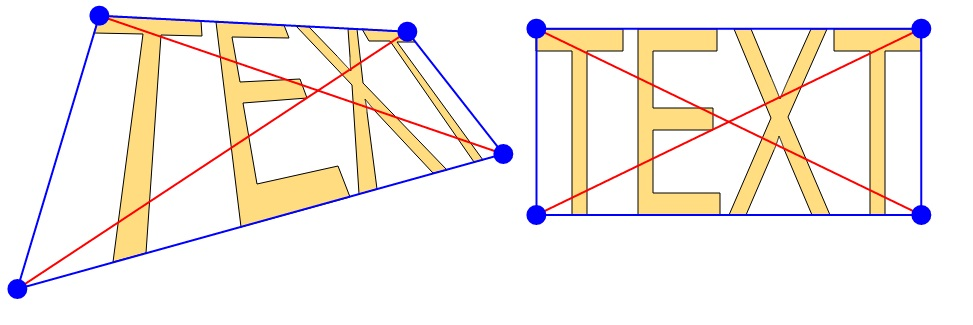
\includegraphics[width=0.9\textwidth]{figures/PersTrans.jpg}
    \label{fig:3.7}
\end{figure}

After finding 4-points which are not linearly dependent, Now we should define the corresponding 4-points to geometrically map the QR-code to a square image. Following code demonstrates the calculation which exactly defines the new corresponding points as "fixed points" and are the Finder patterns and Alignment Pattern places in the standard QR-Matrix which has been defined before.


\begin{lstlisting}

size(ap,2)
if (~isempty(ap) && module>21)      % Versions-1 may not have align pattern
moving_points = [fips(1,2) fips(1,1);            % B position
                    fips(2,2) fips(2,1);            % A position
                        fips(3,2) fips(3,1);        % C position
                            ap(2) ap(1);            % AP 
                            ];

fixed_points = [dist_min dist_fip;
                    dist_min dist_min;
                        dist_fip dist_min;
                              dist_ap dist_ap;
%                              (module)*cell_width (module)*cell_width;
%                              (7)*cell_width (7)*cell_width;
%                              (7)*cell_width (module-7)*cell_width;
%                              (module-7)*cell_width (7)*cell_width;
                            ];

end
       
\end{lstlisting}

Now its the time for MATLAB to transform the perspective by the following prepared function.
\begin{lstlisting}
tform = fitgeotrans(moving_points, fixed_points, 'projective');
newim_S = imwarp(Im, tform, 'linear');
\end{lstlisting}

\subsection{Crop and QR Pattern Demonstration}

After the previous steps, Now we need to crop the QR code pattern from the image and putting it in an exact square form. At first cropping is done by the following part of the program:

\begin{lstlisting}
rect = [FIPLocations(2,2)-(dist_min) FIPLocations(2,1)-(dist_min) side side];
newim = imcrop(newim, rect);
\end{lstlisting}

The using $"imresize"$ function and defining a bigger area(For better demonstration) the QR-code is extracted by the following part of the code:

\begin{lstlisting}
Main_QR_Matrix = imresize(newim, [module module], 'nearest');
Large_QR = imresize(Main_QR_Matrix, [10*module 10*module], 'nearest');
\end{lstlisting}

The following figures show the QR pattern final representation.

\begin{figure}[H]
  \caption{Version-3 QR code recognition}
  \centering
    
\includegraphics[width=0.9\textwidth]{figures/QR1.jpg}
    \label{fig:3.8}
\end{figure}

\begin{figure}[H]
  \caption{Verion-2 QR code}
  \centering
    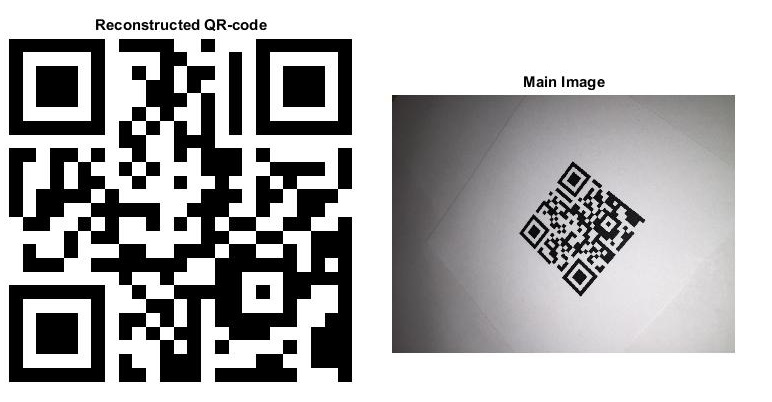
\includegraphics[width=0.9\textwidth]{figures/QR2.jpg}
    \label{fig:3.9}
\end{figure}

\begin{figure}[H]
  \caption{QR code recognition in a high resolution image}
  \centering
    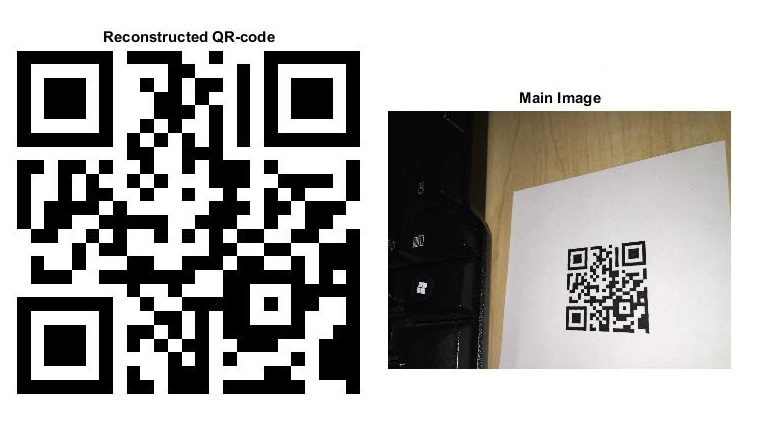
\includegraphics[width=0.9\textwidth]{figures/QR3.jpg}
    \label{fig:3.10}
\end{figure}


This chapter was dedicated to the Image Processing part of the project. In the next chapter decoding of the message will be discussed.







 % Experimental Setup

\lhead{\emph{Decoding and Message Extraction}}
\chapter{Decoding and Message Extraction}

This chapter describes how the data is decoded from the bit streams in order to extracting the message of the QR code. There is two key points which need to be clarified.
\begin{itemize}
\item The first one is we assume that we have the write QR code matrix based on the previous parts. Although some error might be tolerable(regarding the Reed-Solomon error correction) but still we need the QR-Matrix with not much errors.
\item The second one is that if the output message of this part is not correct that doesn't necessary mean that there is some mistakes in the previous parts.
\end{itemize}

The bit stream of the QR-Matrix is the item that connect the image processing part to the decoding part. If the software cannot reconstruct the QR pattern correctly then the decoding part of the software may not be able to decode the message. The flowchart of decoding/message extraction is as what can be seen in the next page.

The developed function $"decode\_ADVANCED\_QR"$, performs the task of decoding and message extraction.



\tikzstyle{decision} = [diamond, draw, fill=blue!20, 
    text width=4.5em, text badly centered, node distance=3cm, inner sep=0pt]
\tikzstyle{block} = [rectangle, draw, fill=blue!20, 
    text width=5em, text centered, rounded corners, minimum height=4em]
\tikzstyle{line} = [draw, -latex']
\tikzstyle{cloud} = [draw, ellipse,fill=red!20, node distance=3cm,
    minimum height=2em]
    
\begin{tikzpicture}[node distance = 3cm, auto]
    % Place nodes
    \node [cloud] (expert) {QR-Matrx};
    \node [block, below of=expert](init) {Decode Format Information};
    \node [cloud, right of=init, node distance=4cm] (system) {Version Num};
    \node [block, below of=init] (identify) {Demasking};
    \node [block, below of=identify] (evaluate) {Reed-Solomon Decoder};
    \node [block, left of=evaluate, node distance=4cm,text width=4cm] (update) {Detect/Correct errors};
    \node [decision, below of=evaluate, node distance=4cm] (decide) {is there any error?};
    \node [block, below of=decide, node distance=4cm,text width=4cm] (AP) {Decode Data Codewords and bit stream};
    \node [decision, right of=AP, node distance=5cm,text width=4cm] (FindAP) {Can you Detect Message Length and Encoding Mode?};
    
    \node [block, right of=FindAP, node distance=5cm] (Geo1) {Extract Final Message};
    \node [block, below of=FindAP, node distance=5cm,text width=4cm] (Geo2) {STOP/Double check Image Processing Part};
   % \node [block, above of=Geo1, node distance=3cm,text %width=4cm] (Crop) {Extract the QR-Code exact image};
 %   \node [block, above of=Crop, node distance=4cm,text %width=4cm] (FF) {Reed-Solomon Decoder/Message Extraction};
    % Draw edges
    \path [line] (init) -- (identify);
    \path [line] (identify) -- (evaluate);
    \path [line] (evaluate) -- (decide);
    \path [line] (decide) -| node [near start] {Yes} (update);
    \path [line,dashed] (update) -- (evaluate);
    \path [line] (decide) -- node {No}(AP);
    \path [line,dashed] (expert) -- (init);
    \path [line,dashed] (system) -- (init);
    \path [line,dashed] (system) |- (identify);
    \path [line] (AP) -- (FindAP);
    \path [line] (FindAP) -- node{Yes}(Geo1);
    \path [line] (FindAP) -- node{No}(Geo2);
    %\draw[ultra thick, blue, ->]  
    %(Geo1) -- (Crop);
    %\draw[ultra thick, blue, ->]  
    %(Geo2) -- (Crop);
    %\draw[ultra thick, red, ->]  
    %(Crop) -- (FF);

   
\end{tikzpicture}

\section{Decoding Data and Final Message}

In this section step by step, the process of decoding the final message will be described according to the previous flowchart. First the positions in the QR matrix which are related to data should be clarified. Using the following code first we put \textbf{"NaN"} in the non-data related positions.

\begin{lstlisting}
referenceIm = false(module);
referenceIm(1:8,1:8) = 1;       % left-upper corner(finder patters)
referenceIm(module-7:module, 1:8) = 1;    % left-down corner(finder patters)
referenceIm(1:8, module-7:module) = 1;    % right-upper corner(finder patters)
if module>21        % version 1 does not have alignment pattern
referenceIm(module-8:module-4,module-8:module-4) = 1;   % Alignment Pattern
end
 referenceIm(7,9:module-8) = 1;      % Horizontal Timing
 referenceIm(9:module-8,7) = 1;      % Vertical Timing
referenceIm(module-7,9) = 1;        % Dark module
\end{lstlisting}

Now we can deal with the other positions as "Data-Related bits".


\subsection{Version and QR code Matrix}

In this part the QR code Matrix and the version are the inputs. The version determines the number of modules in both directions. Since this project is about version 1 through 6 there is no version information in the QR matrix.

\subsection{Format Information Decoding}

In this step the format information which is placed in two
different locations inside the symbol have to be read. As we mentioned before in \ref{Format} there is two bits related to error correction level and three bits related to the number of mask pattern.

To decode the format information, the 15-bits format information should be XORed with the specific 15-bits which mentioned in \ref{Format}. But before XOR operation RS decoding has to be used for detecting and correcting the errors in that 15-bits string. After decoding, the first two bits and next three successive bits determine the error correction level and the number of mask pattern.

\subsection{Demasking}

According to the mask number calculated in the previous part, the matrix should be demasked before entering the Reed-Solomon decoder because in the generating procedure masking in after error correction coding.

\subsection{Reed-Solomon Decoding}

The error correction coding has been used to generate the QR code. Now using RS error correction decoder we need to detect and correct errors. For that first the bit stream should be converted to a decimal sequence to be used in Reed-Solomon decoder. RS decoder is an object which is provided within the "Communication Systems Toolbox" in MATLAB. Although it is provided by MATLAB but implementing it is not a trivial task. The script for Reed-Solomon decoding is as below:
\begin{lstlisting}
function [ str_decode ] = Reed_SLM_Decoder( msg,ECC )

m = 8; % Number of bits in each symbol
n = 2^m-1; k = n-length(ECC); % Codeword length and message length
hDec = comm.RSDecoder(n,k);
release(hDec)
hDec.GeneratorPolynomialSource = 'Property';
hDec.GeneratorPolynomial       = rsgenpoly(n,k,[],0);
c2 = [zeros(1,n-length(msg)-length(ECC)) msg ECC]';
d2 = step(hDec, c2);
d=d2(size(d2,1)-length(msg)+1:size(d2,1),1);
d=d';
str_decode=d;
end
\end{lstlisting}

Note that although RS codes are symmetric but we cannot use RS decoder directly because for the generation part there are different interleaving patterns for encoding the data and error correction codewords. refer to \cite{1iso} for more information.

\subsection{Message Extraction}

The corrected data codewords which have to be placed in the correct order should be converted in a binary bit stream. The first four bits indicate the mode that is used to
represent the codewords in bit sequence. Then the next 8 or 9 or  etc bits(depends on the encoding mode) demonstrate the message length. Finally by considering the procedure which mentioned in \ref{Encod} the message extraction should be done.

It is useful to demonstrate some results and final message of different test images to better following the results.


\begin{figure}[H]
     \begin{center}
%
        \subfigure[Verions-3 Qr code Message Extraction]{%
            \label{fig:first}
            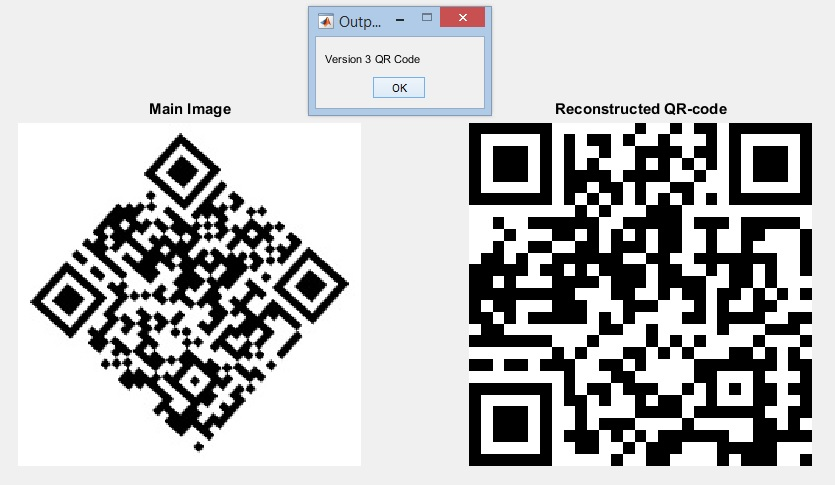
\includegraphics[width=0.9\textwidth]{figures/decod1.jpg}
        }\\%
        \subfigure[Verions-2 Qr High-resolution code]{%
           \label{fig:second}
           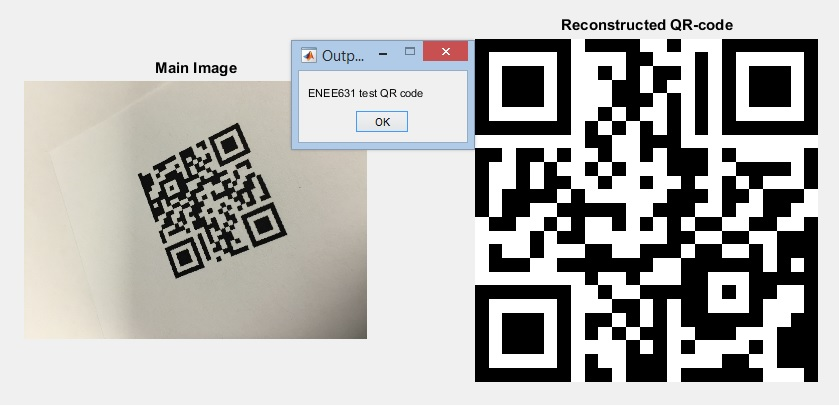
\includegraphics[width=0.9\textwidth]{figures/decod2.jpg}
        }\\%  ------- End of the first row 
        \subfigure[Verions-2 Qr code side view]{%
           \label{fig:second}
           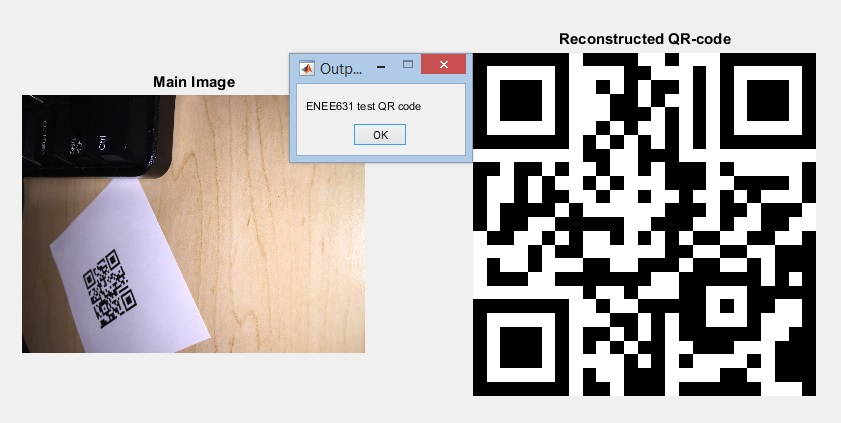
\includegraphics[width=0.9\textwidth]{figures/decod3.jpg}
        }
    \end{center}
    \caption{%
Message extraction of Version-2 and Version-3
     }%
   \label{fig4.1}
\end{figure}

\newpage
Now it is interesting to decode a QR doce from higher version. The following image is a version-5 QR code.

\begin{figure}[H]
  \caption{Version-5 QR code message extraction}
  \centering
    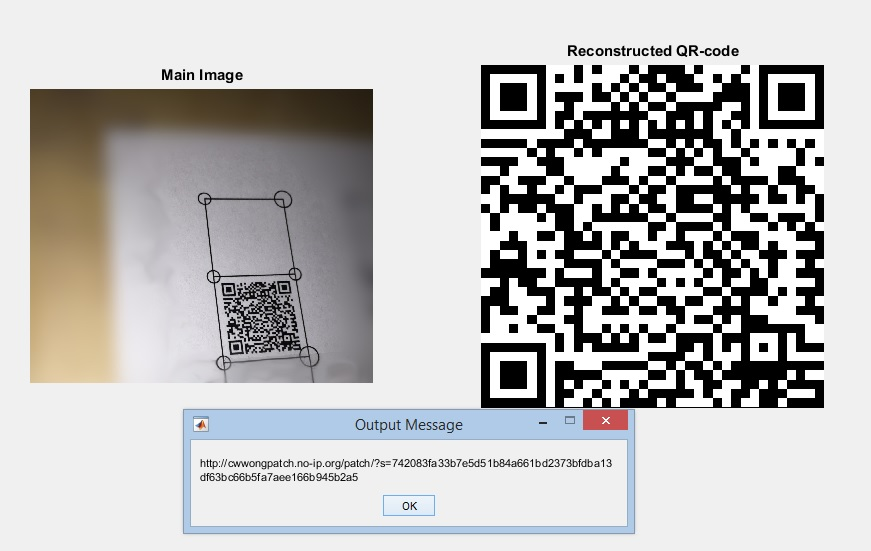
\includegraphics[width=0.9\textwidth]{figures/decod4.jpg}
    \label{fig:4.2}
\end{figure}

In this chapter the final part which is decoding and demonstrating the message has been described in detail and results were shown. Next chapter is the conclusion of the project and provides some discussions about the alternative approaches and deficiencies.
 % QR Code Structure
\clearpage

\lhead{\emph{Conclusion and Discussion}}
\chapter{Conclusion and Discussion}

This aim of this chapter is to provide some discussion about results, as the speed and reliability point of view. Some suggestion has been provided in the end.

\section{Speed}

The following table provides some number in order to better understanding the effect of matrices size and version number on the algorithm.

\begin{table}[h!]
  \centering
          \caption{Effect of number of pixels and version number on the speed}
         \label{table5.1}
    \begin{tabular}{| l | l | l | l |}
    \hline
    Image-Num & Number of pixels & Runtime(Sec) & Version Number \\ \hline
    Image-1 & $220\times220$ & 1.59 & 3  \\ \hline
    Image-2 & $2448\times3264$ & 9.5 & 2  \\ \hline
    Image-3 & $2448\times3264$ & 9.7 & 2  \\ \hline
    Image-4 & $686\times607$ & 3.2 & 3  \\ \hline
    Image-5 & $2448\times2100$ & 7.85 & 5  \\ \hline
    \end{tabular}

\end{table}

As it can be seen from the table \ref{table5.1} Image-2 and Image-3 has the same size and are from the same version but the simulation time is a little higher in Image-3. The reason is that for any reason the Image-3 size is more than Image-2 in Byte and it related to the JPEG compression.

Another interesting point is that also Image-5 is smaller than Image-2 but the run-time is not very different because the Image-5 is from version-5 and it concludes to higher complexity during the simulation procedure.

\section{Reliability}

The reliability is based on two important consideration:

\begin{itemize}
\item The first one is that whether the image processing part can extract the correct QR pattern or not?

\item The second one is that is we have the correct pattern of the QR code, whether we can decode it or not?
\end{itemize}

\subsection{Error Correction Reliability}
The second item related to the number of errors which Reed-Solomon decoder should correct. If the error is more than the maximum ability of the error correction then the message cannot be correctly and fully decoded. Since this part is not the main goal of this project/course so we don't go deep any further in this area.

\subsection{QR Code Pattern Recognition Ability}

There is different scenarios and different approaches to overcome the deficiencies. We investigate them from the easy to the worst case scenario.

\subsubsection{Three Finder Pattern and one Alignment Pattern}

Suppose that we have a clear image and straight point of view. This is the easiest scenario. We believe that the software can easily detect the finder patterns and alignment pattern and the QR code reconstruction would be easy. In other scenarios even if the image is blurred or damaged, if we can find this 4-points, then we can perfectly reconstruct the QR code.

\textbf{Limitation} \\

The caveat is that what if the simulation finds a wrong alignment pattern or finder patter? The answer is according to the characteristics of the finder patter it is very unlikely to find a wrong finder pattern. The software has been tested for wide variety of images. The problem is that it is likely for software to find a point as the Alignment Pattern while it is not!! The reason that we have add another diagonal ration search for AP candidates is to prevent this phenomenon and by testing different test images we conclude that the developed software is reliable to that even.

\subsubsection{Three Finder Pattern and no Alignment Pattern}

Sometimes the software cannot find the AP because there might be no AP in a damaged image or there is but the software cannot be find the Alignment Pattern. The former has no solution for finding AP but for the later we can allow more error in searching for the alignment pattern. This ability is defined in the software. 

\textbf{Limitation} \\

The caveat is that allowing more error might lead to finding an Alignment Pattern which is not the correct one. The final solution for that which prevent this issue is that if the software cannot detect AP then ignore it and use the last corner of the QR-Code as the fourth point for perspective transformation. But the previous algorithm that we developed for this task was not very precise because if the image is not from straight point of view the if the looking angle is far from 90 even by 20 degree, then the software fail to find the fourth corner of the QR-Code\footnote{Fourth corner refers to the corner which is not connected to any of three finder patterns} pattern. In better words it finds something which is not the correct one. The last algorithm that we implemented for this issue is to find two candidates for the fourth corner and using the average. According to the test images that we used for this algorithm, it is more efficient than the previous one.

\subsubsection{Less Than Three Finder Pattern}

If the simulation cannot find more than three finder pattern then it is very difficult to tackle this problem. It may happen in very rare scenarios which the image is very blurred and almost the pattern cannot be scene. The solution is to use different thresholding in order to find and locate the finder patterns and separators. In this scenario we try the previous approach for finding the fourth corner of QR code and try to reconstruct the pattern.

\subsubsection{Advantage of Algorithm for Finding the Fourth Corner}

The advantage of finding the fourth corner is that is lots of the scenarios we can have a straight image from the pattern whether blurred and noisy or not. Using this method we don't need to have the Alignment Pattern location. It might be less reliable but if there is not any other choice it can be applied.
\section{Limitation of Decoding}

The simulation sometimes fails to decode the version 5-Q and 5-H QR code because of the more complex interleaving pattern of the data and error correction code-words. The author is working on modifying the software to successfully decode 5-Q and 5-H QR codes.

\section{Future work}

Since this project is only considering the version 1 through 6 then an interesting extend to this project can be modifying software for having correct results for higher versions.

Since the version number should be enter by the software executive man another interesting extend can be developing a software to automatically detect the version of QR-Code which is a practical task and can be well implemented in real life applications.

The other issue to finding the alignment pattern. The software should be adapted such that if there is any Alignment pattern it has the reliability to locate that. Basically our software do the job quite well but testing its reliability in deeper sense can improve its efficiency. % QR Code Structure
\clearpage
%\chapter{Decoding and Message Extraction}

This chapter describes how the data is decoded from the bit streams in order to extracting the message of the QR code. There is two key points which need to be clarified.
\begin{itemize}
\item The first one is we assume that we have the write QR code matrix based on the previous parts. Although some error might be tolerable(regarding the Reed-Solomon error correction) but still we need the QR-Matrix with not much errors.
\item The second one is that if the output message of this part is not correct that doesn't necessary mean that there is some mistakes in the previous parts.
\end{itemize}

The bit stream of the QR-Matrix is the item that connect the image processing part to the decoding part. If the software cannot reconstruct the QR pattern correctly then the decoding part of the software may not be able to decode the message. The flowchart of decoding/message extraction is as what can be seen in the next page.

The developed function $"decode\_ADVANCED\_QR"$, performs the task of decoding and message extraction.



\tikzstyle{decision} = [diamond, draw, fill=blue!20, 
    text width=4.5em, text badly centered, node distance=3cm, inner sep=0pt]
\tikzstyle{block} = [rectangle, draw, fill=blue!20, 
    text width=5em, text centered, rounded corners, minimum height=4em]
\tikzstyle{line} = [draw, -latex']
\tikzstyle{cloud} = [draw, ellipse,fill=red!20, node distance=3cm,
    minimum height=2em]
    
\begin{tikzpicture}[node distance = 3cm, auto]
    % Place nodes
    \node [cloud] (expert) {QR-Matrx};
    \node [block, below of=expert](init) {Decode Format Information};
    \node [cloud, right of=init, node distance=4cm] (system) {Version Num};
    \node [block, below of=init] (identify) {Demasking};
    \node [block, below of=identify] (evaluate) {Reed-Solomon Decoder};
    \node [block, left of=evaluate, node distance=4cm,text width=4cm] (update) {Detect/Correct errors};
    \node [decision, below of=evaluate, node distance=4cm] (decide) {is there any error?};
    \node [block, below of=decide, node distance=4cm,text width=4cm] (AP) {Decode Data Codewords and bit stream};
    \node [decision, right of=AP, node distance=5cm,text width=4cm] (FindAP) {Can you Detect Message Length and Encoding Mode?};
    
    \node [block, right of=FindAP, node distance=5cm] (Geo1) {Extract Final Message};
    \node [block, below of=FindAP, node distance=5cm,text width=4cm] (Geo2) {STOP/Double check Image Processing Part};
   % \node [block, above of=Geo1, node distance=3cm,text %width=4cm] (Crop) {Extract the QR-Code exact image};
 %   \node [block, above of=Crop, node distance=4cm,text %width=4cm] (FF) {Reed-Solomon Decoder/Message Extraction};
    % Draw edges
    \path [line] (init) -- (identify);
    \path [line] (identify) -- (evaluate);
    \path [line] (evaluate) -- (decide);
    \path [line] (decide) -| node [near start] {Yes} (update);
    \path [line,dashed] (update) -- (evaluate);
    \path [line] (decide) -- node {No}(AP);
    \path [line,dashed] (expert) -- (init);
    \path [line,dashed] (system) -- (init);
    \path [line,dashed] (system) |- (identify);
    \path [line] (AP) -- (FindAP);
    \path [line] (FindAP) -- node{Yes}(Geo1);
    \path [line] (FindAP) -- node{No}(Geo2);
    %\draw[ultra thick, blue, ->]  
    %(Geo1) -- (Crop);
    %\draw[ultra thick, blue, ->]  
    %(Geo2) -- (Crop);
    %\draw[ultra thick, red, ->]  
    %(Crop) -- (FF);

   
\end{tikzpicture}

\section{Decoding Data and Final Message}

In this section step by step, the process of decoding the final message will be described according to the previous flowchart. First the positions in the QR matrix which are related to data should be clarified. Using the following code first we put \textbf{"NaN"} in the non-data related positions.

\begin{lstlisting}
referenceIm = false(module);
referenceIm(1:8,1:8) = 1;       % left-upper corner(finder patters)
referenceIm(module-7:module, 1:8) = 1;    % left-down corner(finder patters)
referenceIm(1:8, module-7:module) = 1;    % right-upper corner(finder patters)
if module>21        % version 1 does not have alignment pattern
referenceIm(module-8:module-4,module-8:module-4) = 1;   % Alignment Pattern
end
 referenceIm(7,9:module-8) = 1;      % Horizontal Timing
 referenceIm(9:module-8,7) = 1;      % Vertical Timing
referenceIm(module-7,9) = 1;        % Dark module
\end{lstlisting}

Now we can deal with the other positions as "Data-Related bits".


\subsection{Version and QR code Matrix}

In this part the QR code Matrix and the version are the inputs. The version determines the number of modules in both directions. Since this project is about version 1 through 6 there is no version information in the QR matrix.

\subsection{Format Information Decoding}

In this step the format information which is placed in two
different locations inside the symbol have to be read. As we mentioned before in \ref{Format} there is two bits related to error correction level and three bits related to the number of mask pattern.

To decode the format information, the 15-bits format information should be XORed with the specific 15-bits which mentioned in \ref{Format}. But before XOR operation RS decoding has to be used for detecting and correcting the errors in that 15-bits string. After decoding, the first two bits and next three successive bits determine the error correction level and the number of mask pattern.

\subsection{Demasking}

According to the mask number calculated in the previous part, the matrix should be demasked before entering the Reed-Solomon decoder because in the generating procedure masking in after error correction coding.

\subsection{Reed-Solomon Decoding}

The error correction coding has been used to generate the QR code. Now using RS error correction decoder we need to detect and correct errors. For that first the bit stream should be converted to a decimal sequence to be used in Reed-Solomon decoder. RS decoder is an object which is provided within the "Communication Systems Toolbox" in MATLAB. Although it is provided by MATLAB but implementing it is not a trivial task. The script for Reed-Solomon decoding is as below:
\begin{lstlisting}
function [ str_decode ] = Reed_SLM_Decoder( msg,ECC )

m = 8; % Number of bits in each symbol
n = 2^m-1; k = n-length(ECC); % Codeword length and message length
hDec = comm.RSDecoder(n,k);
release(hDec)
hDec.GeneratorPolynomialSource = 'Property';
hDec.GeneratorPolynomial       = rsgenpoly(n,k,[],0);
c2 = [zeros(1,n-length(msg)-length(ECC)) msg ECC]';
d2 = step(hDec, c2);
d=d2(size(d2,1)-length(msg)+1:size(d2,1),1);
d=d';
str_decode=d;
end
\end{lstlisting}

Note that although RS codes are symmetric but we cannot use RS decoder directly because for the generation part there are different interleaving patterns for encoding the data and error correction codewords. refer to \cite{1iso} for more information.

\subsection{Message Extraction}

The corrected data codewords which have to be placed in the correct order should be converted in a binary bit stream. The first four bits indicate the mode that is used to
represent the codewords in bit sequence. Then the next 8 or 9 or  etc bits(depends on the encoding mode) demonstrate the message length. Finally by considering the procedure which mentioned in \ref{Encod} the message extraction should be done.

It is useful to demonstrate some results and final message of different test images to better following the results.


\begin{figure}[H]
     \begin{center}
%
        \subfigure[Verions-3 Qr code Message Extraction]{%
            \label{fig:first}
            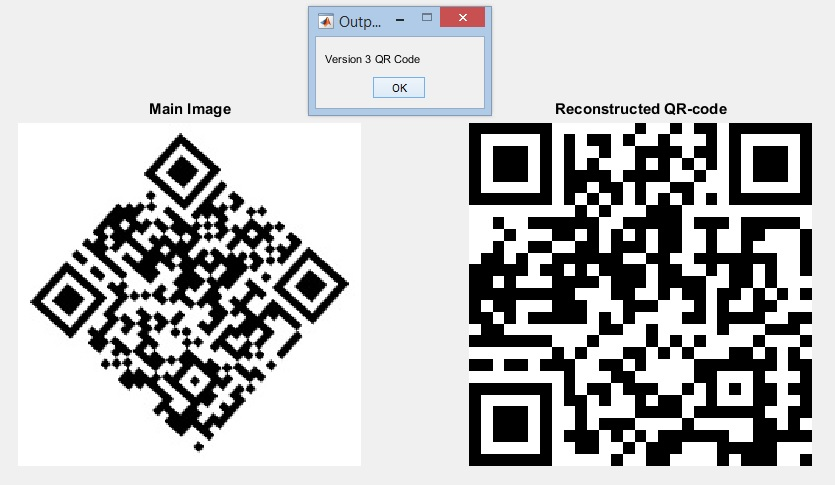
\includegraphics[width=0.9\textwidth]{figures/decod1.jpg}
        }\\%
        \subfigure[Verions-2 Qr High-resolution code]{%
           \label{fig:second}
           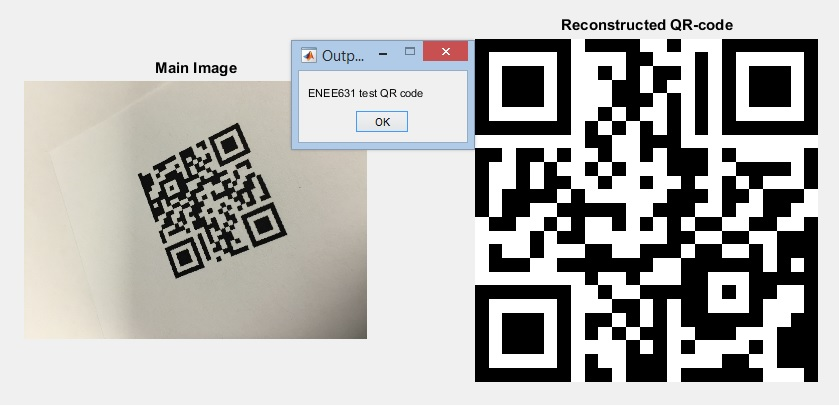
\includegraphics[width=0.9\textwidth]{figures/decod2.jpg}
        }\\%  ------- End of the first row 
        \subfigure[Verions-2 Qr code side view]{%
           \label{fig:second}
           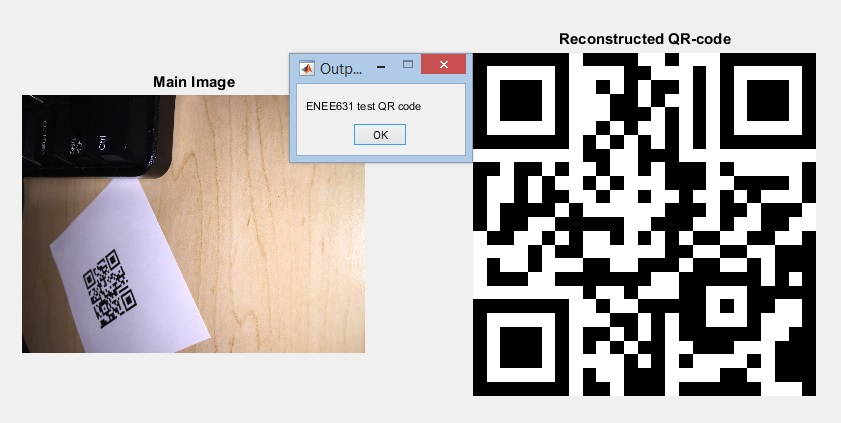
\includegraphics[width=0.9\textwidth]{figures/decod3.jpg}
        }
    \end{center}
    \caption{%
Message extraction of Version-2 and Version-3
     }%
   \label{fig4.1}
\end{figure}

\newpage
Now it is interesting to decode a QR doce from higher version. The following image is a version-5 QR code.

\begin{figure}[H]
  \caption{Version-5 QR code message extraction}
  \centering
    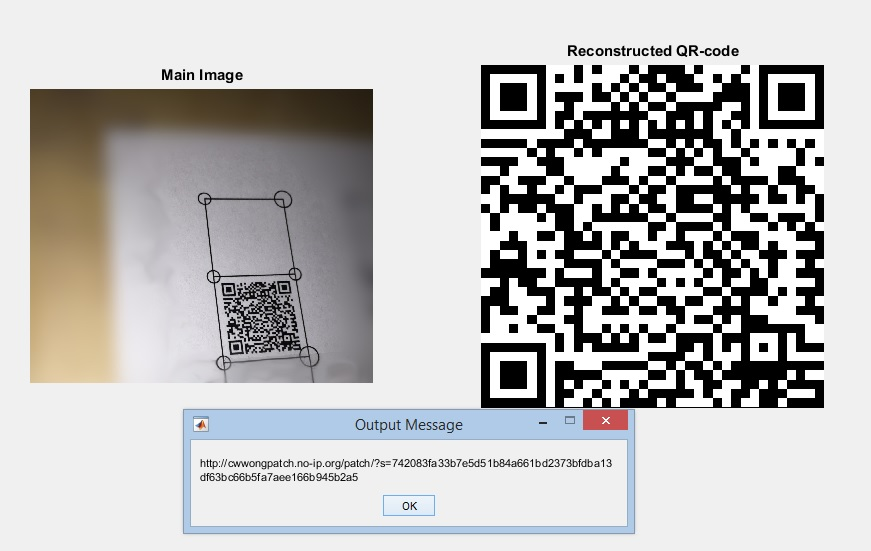
\includegraphics[width=0.9\textwidth]{figures/decod4.jpg}
    \label{fig:4.2}
\end{figure}

In this chapter the final part which is decoding and demonstrating the message has been described in detail and results were shown. Next chapter is the conclusion of the project and provides some discussions about the alternative approaches and deficiencies.
 % Experiment 1

%\chapter{Conclusion and Discussion}

This aim of this chapter is to provide some discussion about results, as the speed and reliability point of view. Some suggestion has been provided in the end.

\section{Speed}

The following table provides some number in order to better understanding the effect of matrices size and version number on the algorithm.

\begin{table}[h!]
  \centering
          \caption{Effect of number of pixels and version number on the speed}
         \label{table5.1}
    \begin{tabular}{| l | l | l | l |}
    \hline
    Image-Num & Number of pixels & Runtime(Sec) & Version Number \\ \hline
    Image-1 & $220\times220$ & 1.59 & 3  \\ \hline
    Image-2 & $2448\times3264$ & 9.5 & 2  \\ \hline
    Image-3 & $2448\times3264$ & 9.7 & 2  \\ \hline
    Image-4 & $686\times607$ & 3.2 & 3  \\ \hline
    Image-5 & $2448\times2100$ & 7.85 & 5  \\ \hline
    \end{tabular}

\end{table}

As it can be seen from the table \ref{table5.1} Image-2 and Image-3 has the same size and are from the same version but the simulation time is a little higher in Image-3. The reason is that for any reason the Image-3 size is more than Image-2 in Byte and it related to the JPEG compression.

Another interesting point is that also Image-5 is smaller than Image-2 but the run-time is not very different because the Image-5 is from version-5 and it concludes to higher complexity during the simulation procedure.

\section{Reliability}

The reliability is based on two important consideration:

\begin{itemize}
\item The first one is that whether the image processing part can extract the correct QR pattern or not?

\item The second one is that is we have the correct pattern of the QR code, whether we can decode it or not?
\end{itemize}

\subsection{Error Correction Reliability}
The second item related to the number of errors which Reed-Solomon decoder should correct. If the error is more than the maximum ability of the error correction then the message cannot be correctly and fully decoded. Since this part is not the main goal of this project/course so we don't go deep any further in this area.

\subsection{QR Code Pattern Recognition Ability}

There is different scenarios and different approaches to overcome the deficiencies. We investigate them from the easy to the worst case scenario.

\subsubsection{Three Finder Pattern and one Alignment Pattern}

Suppose that we have a clear image and straight point of view. This is the easiest scenario. We believe that the software can easily detect the finder patterns and alignment pattern and the QR code reconstruction would be easy. In other scenarios even if the image is blurred or damaged, if we can find this 4-points, then we can perfectly reconstruct the QR code.

\textbf{Limitation} \\

The caveat is that what if the simulation finds a wrong alignment pattern or finder patter? The answer is according to the characteristics of the finder patter it is very unlikely to find a wrong finder pattern. The software has been tested for wide variety of images. The problem is that it is likely for software to find a point as the Alignment Pattern while it is not!! The reason that we have add another diagonal ration search for AP candidates is to prevent this phenomenon and by testing different test images we conclude that the developed software is reliable to that even.

\subsubsection{Three Finder Pattern and no Alignment Pattern}

Sometimes the software cannot find the AP because there might be no AP in a damaged image or there is but the software cannot be find the Alignment Pattern. The former has no solution for finding AP but for the later we can allow more error in searching for the alignment pattern. This ability is defined in the software. 

\textbf{Limitation} \\

The caveat is that allowing more error might lead to finding an Alignment Pattern which is not the correct one. The final solution for that which prevent this issue is that if the software cannot detect AP then ignore it and use the last corner of the QR-Code as the fourth point for perspective transformation. But the previous algorithm that we developed for this task was not very precise because if the image is not from straight point of view the if the looking angle is far from 90 even by 20 degree, then the software fail to find the fourth corner of the QR-Code\footnote{Fourth corner refers to the corner which is not connected to any of three finder patterns} pattern. In better words it finds something which is not the correct one. The last algorithm that we implemented for this issue is to find two candidates for the fourth corner and using the average. According to the test images that we used for this algorithm, it is more efficient than the previous one.

\subsubsection{Less Than Three Finder Pattern}

If the simulation cannot find more than three finder pattern then it is very difficult to tackle this problem. It may happen in very rare scenarios which the image is very blurred and almost the pattern cannot be scene. The solution is to use different thresholding in order to find and locate the finder patterns and separators. In this scenario we try the previous approach for finding the fourth corner of QR code and try to reconstruct the pattern.

\subsubsection{Advantage of Algorithm for Finding the Fourth Corner}

The advantage of finding the fourth corner is that is lots of the scenarios we can have a straight image from the pattern whether blurred and noisy or not. Using this method we don't need to have the Alignment Pattern location. It might be less reliable but if there is not any other choice it can be applied.
\section{Limitation of Decoding}

The simulation sometimes fails to decode the version 5-Q and 5-H QR code because of the more complex interleaving pattern of the data and error correction code-words. The author is working on modifying the software to successfully decode 5-Q and 5-H QR codes.

\section{Future work}

Since this project is only considering the version 1 through 6 then an interesting extend to this project can be modifying software for having correct results for higher versions.

Since the version number should be enter by the software executive man another interesting extend can be developing a software to automatically detect the version of QR-Code which is a practical task and can be well implemented in real life applications.

The other issue to finding the alignment pattern. The software should be adapted such that if there is any Alignment pattern it has the reliability to locate that. Basically our software do the job quite well but testing its reliability in deeper sense can improve its efficiency. % Experiment 2

%\input{Chapters/Chapter6} % Results and Discussion

%\input{Chapters/Chapter7} % Conclusion

%% ----------------------------------------------------------------
% Now begin the Appendices, including them as separate files

\addtocontents{toc}{\vspace{2em}} % Add a gap in the Contents, for aesthetics

\appendix % Cue to tell LaTeX that the following 'chapters' are Appendices

%\chapter{An Appendix}

Lorem ipsum dolor sit amet, consectetur adipiscing elit. Vivamus 	% Appendix Title

%\input{Appendices/AppendixB} % Appendix Title

%\input{Appendices/AppendixC} % Appendix Title

\addtocontents{toc}{\vspace{2em}}  % Add a gap in the Contents, for aesthetics
\backmatter

%% ----------------------------------------------------------------






\label{Bibliography}
\lhead{\emph{Bibliography}}  % Change the left side page header to "Bibliography"
\bibliographystyle{plain}  % Use the "unsrtnat" BibTeX style for formatting the Bibliography
%\bibliography{Bibliography}  % The references (bibliography) information are stored in the file named "Bibliography.bib"
\begin{thebibliography}{9}

\bibitem{1iso}
ISO/IEC 18004. Information technology - Automatic identification and data capture
techniques - QR code 2005 bar code symbology specification. \textit{International Standard}, (Second Edition), September 2006. URL \url{http://www.iso.org}.

\bibitem{Thonky}
qr-code-tutorial. URL \url{www.thonky.com/qr-code-tutorial}.

\bibitem{WikiHomo}
Wikipedia: Homography. URL \url{http://en.wikipedia.org/wiki/Projective_transformation}.

\bibitem{StackPers}
Stackoverflor: Perspective Transformation. URL \url{stackoverflow.com}.

\end{thebibliography}






%%%%%%%%%%%%%%%%%%%%%%%%%%%%%%%%%%
%%%%%%%%%%%%%%%%%%%%%%%%%%%%%%%%%
%%%%%%%%%%%%%%%%%%%%%%%%%%%%%%%%%%
\end{document}  % The End
%% ----------------------------------------------------------------